\documentclass[10pt]{article}

% amsmath package, useful for mathematical formulas
\usepackage{amsmath}
% amssymb package, useful for mathematical symbols
\usepackage{amssymb}

% graphicx package, useful for including eps and pdf graphics
% include graphics with the command \includegraphics
\usepackage{graphicx}

% cite package, to clean up citations in the main text. Do not remove.
\usepackage{cite}

\usepackage{color} 

% Use doublespacing - comment out for single spacing
%\usepackage{setspace} 
%\doublespacing


% Text layout
\topmargin 0.0cm
\oddsidemargin 0.5cm
\evensidemargin 0.5cm
\textwidth 16cm 
\textheight 21cm

% Bold the 'Figure #' in the caption and separate it with a period
% Captions will be left justified
\usepackage[labelfont=bf,labelsep=period,justification=raggedright]{caption}

% Use the PLoS provided bibtex style
\bibliographystyle{PLoS2009}

% Remove brackets from numbering in List of References
\makeatletter
\renewcommand{\@biblabel}[1]{\quad#1.}
\makeatother


% Leave date blank
\date{}

\pagestyle{myheadings}
%% ** EDIT HERE **
%% Please insert a running head of 30 characters or less.  
%% Include it twice, once between each set of braces
\markboth{Modeling structured RNA}{Modeling structured RNA}

%% ** EDIT HERE **
%% PLEASE INCLUDE ALL MACROS BELOW
\usepackage{setspace}
\doublespacing

%parsetree.sty - LaTeX style file with macros for typesetting parse trees
% See parsetree.doc for extensive section-by-section comments to the code.
% Eirik Hektoen, 1994-2-24

\typeout{Including style file `parsetree.sty'.}


% Some Initial Variables and Auxiliary Macros:

\def\pterror#1{\errmessage{Parsetree ERROR: #1}}

\newdimen\pthgap\def\pthorgap#1{\pthgap=#1}
\newdimen\ptvgap\def\ptvergap#1{\ptvgap=#1}

\newbox\ptnodestrutbox\def\ptnodestrut{\unhcopy\ptnodestrutbox}
\newbox\ptleafstrutbox\def\ptleafstrut{\unhcopy\ptleafstrutbox}

\def\ptnodefont#1#2#3{\def\ptnodefn{#1}
  \setbox\ptnodestrutbox=\hbox{\vrule height#2 width0pt depth#3}}
\def\ptleaffont#1#2#3{\def\ptleaffn{#1}
  \setbox\ptleafstrutbox=\hbox{\vrule height#2 width0pt depth#3}}


% Customizable Definitions (- NOTE: MAY BE REDEFINED IN DOCUMENT -):

\pthorgap{12pt}                         % horizontal gap betw sisters
\ptvergap{12pt}                         % vertical gap betw mother/daughter
\ptnodefont{\normalsize\rm}{11pt}{3pt}  % font and strut height/depth: nodes
\ptleaffont{\normalsize\it}{11pt}{3pt}  % font and strut height/depth: leaves


% Hierarchy-building macros:

\newcount\ptdepth           % current bracketing depth
\newcount\ptn               % 1: m, 2: ma, 3: mab, 4: mabc
\newbox\ptm \newdimen\ptmx  % m = mother
\newbox\pta \newdimen\ptax  % a = 1st daughter
\newbox\ptb \newdimen\ptbx  % b = 2nd daughter
\newbox\ptc \newdimen\ptcx  % c = 3rd daughter (max)
\newbox\ptx \newdimen\ptxx  % x = used for passing results
\newif\ifpttri              % choose triangular subtree with \pttritrue

\def\ptnext{\advance\ptn by 1 \ifcase\ptn
  \or \setbox\ptm=\box\ptx \ptmx=\ptxx \or \setbox\pta=\box\ptx \ptax=\ptxx
  \or \setbox\ptb=\box\ptx \ptbx=\ptxx \or \setbox\ptc=\box\ptx \ptcx=\ptxx
  \else \pterror{More than 3 daughters in (sub)tree}\fi}

\def\ptbegtree{\ptdepth=0}
\def\ptendtree
  {\ifnum\ptdepth>0 \pterror{Mismatched bracketing: too few ')'s!}\fi}

\def\ptbeg{\ifnum\ptdepth=0 \leavevmode\fi\begingroup
  \advance\ptdepth1 \ptn=0\pttrifalse}
\def\ptend{\ifnum\ptdepth=0 \pterror{Mismatched bracketing: too many ')'s!}
  \else\ptcons\endgroup\ifnum\ptdepth=0 \box\ptx\else\ptnext\fi\fi}

\def\ptnodeaux#1{\setbox\ptx=\hbox{#1}\ptxx=0.5\wd\ptx\ptnext}
\def\ptnode#1{\ptnodeaux{\ptnodefn\ptnodestrut #1}}
\def\ptleaf#1{\ptnodeaux{\ptleaffn\ptleafstrut #1}}

\def\pthoradjust#1{\ifcase\ptn
  \or \pthadjbox{\ptm}{#1} \or \pthadjbox{\pta}{#1}
  \or \pthadjbox{\ptb}{#1} \or \pthadjbox{\ptc}{#1}
  \else \pterror{More than 3 daughters in (sub)tree}\fi}
\def\pthadjbox#1#2{\setbox#1=\hbox{\box#1\kern#2}}


% Subtree-constructing macros:

\def\ptcons
 {\ifnum\ptn=0 \ptconsz 
  \else
    \ifpttri\ptconstri\else
      \ifcase\ptn \or\ptconsm\or\ptconsma\or\ptconsmab\or\ptconsmabc \fi \fi
    \ptax=\ptxx \advance\ptax-\ptmx \ptbx=0pt
    \ifdim\ptax<0pt \ptbx=-\ptax\ptax=0pt\ptxx=\ptmx \fi
    \setbox\ptx=\vtop{\hbox{\kern\ptax\box\ptm}\nointerlineskip
                      \hbox{\kern\ptbx\box\ptx}}\fi
  \global\ptxx=\ptxx\global\setbox\ptx=\box\ptx}

\def\ptavg#1#2#3{#1=#2\advance#1#3#1=0.5#1}     % #1 := average(#2,#3)
\def\ptadv#1#2{\advance#1#2\advance#1\pthgap}   % #1 := #1 + #2 + \pthgap

\def\ptconsz{\ptxx=0pt \setbox\ptx=\vtop{}}     % empty (zero) tree

\def\ptconsm{\ptxx=0pt 
  \setbox\ptx=\hbox{\ptedge{1}{0}{}{}}}         % mother only

\def\ptconsma                                   % mother and one daughter
 {\ptxx=\ptax\setbox\ptx=\vtop{
    \hbox{\ptedge{1}\ptax{}{}}\nointerlineskip
    \hbox{\box\pta}}}

\def\ptconsmab                                  % mother and two daughters
 {\ptadv\ptbx{\wd\pta}\ptavg\ptxx\ptax\ptbx
  \setbox\ptx=\vtop{
    \hbox{\ptedge{2}\ptax\ptbx{}}\nointerlineskip
    \hbox{\box\pta\kern\pthgap\box\ptb}}}

\def\ptconsmabc                                 % mother and three daughters
 {\ptadv\ptbx{\wd\pta}\ptadv\ptcx{\wd\pta}%
  \ptadv\ptcx{\wd\ptb}\ptavg\ptxx\ptax\ptcx
  \setbox\ptx=\vtop{
    \hbox{\ptedge{3}\ptax\ptbx\ptcx}\nointerlineskip
    \hbox{\box\pta\kern\pthgap\box\ptb\kern\pthgap\box\ptc}}}

\def\ptconstri                                  % triangular subtree
 {\ifcase\ptn\or\setbox\pta\hbox{\kern2\pthgap}\or
  \or\setbox\pta=\hbox{\box\pta\kern\pthgap\box\ptb}
  \or\setbox\pta=\hbox{\box\pta\kern\pthgap\box\ptb\kern\pthgap\box\ptc}\fi
  \ptxx=0.5\wd\pta
  \setbox\ptx=\vtop{
    \hbox{\ptedge{0}{0}{\wd\pta}{}}\nointerlineskip
    \box\pta}}


% Macros for `diagonal rules':

\newcount\pted          % edge mode
\newcount\ptedm         % position of mother
\newcount\pteda         % position a
\newcount\ptedb         % position b
\newcount\ptedc         % position c
\newcount\ptedl         % edge length
\newcount\ptedh         % edge height
\newcount\ptedhs        % horizontal slope
\newcount\ptedvs        % vertical slope
\newcount\ptedtemp      % temporary variable

\def\ptedge#1#2#3#4{\pted=#1%
  \pteda=#2\ifcase\pted\ptedb=#3\or\or\ptedb=#3\or\ptedb=#3\ptedc=#4\fi
  \ptedm=\pteda\advance\ptedm\ifcase\pted\ptedb\or\pteda\or\ptedb\or\ptedc\fi
  \divide\ptedm by 2
  \ptedh=\ptvgap\ptedtemp=\ptedm\advance\ptedtemp-\pteda\divide\ptedtemp by 6
  \ifnum\ptedh<\ptedtemp\ptedh=\ptedtemp\fi
  \unitlength=1sp%
  \begin{picture}(0,\ptedh)
    \ifnum\pted=3 \ptedput\ptedc\fi
    \ifnum\pted=1 \else\ptedput\ptedb\fi
    \ptedput\pteda
    \ifnum\pted=0 \ptedbot\fi 
  \end{picture}}

\def\ptedput#1{\ptedl=#1\advance\ptedl-\ptedm
  \ifnum\ptedl>0 \ptedslope\else
    \ptedl=-\ptedl\ptedslope\ptedhs=-\ptedhs\fi
  \ifnum\ptedhs=0 \ptedl=\ptedh\fi
  \put(\ptedm,\ptedh){\line(\ptedhs,-\ptedvs){\ptedl}}}

\def\ptedbot
 {\ptedtemp=\ptedl\multiply\ptedtemp by \ptedvs\divide\ptedtemp by \ptedhs
  \ifnum\ptedtemp>0\ptedtemp=-\ptedtemp\fi \advance\ptedtemp-1
  \advance\ptedtemp\ptedh\multiply\ptedl by 2
  \put(\pteda,\ptedtemp){\line(1,0){\ptedl}}}

\def\ptedslope
 {\ifnum\ptedl>\ptedh\ptedhs=\ptedl\ptedvs=\ptedh
  \else              \ptedvs=\ptedl\ptedhs=\ptedh \fi
  \divide\ptedhs by 60 \divide\ptedvs by \ptedhs
  \ifnum \ptedvs <  5 \ptedvs=0 \ptedhs=1 \else
  \ifnum \ptedvs < 11 \ptedvs=1 \ptedhs=6 \else
  \ifnum \ptedvs < 13 \ptedvs=1 \ptedhs=5 \else
  \ifnum \ptedvs < 17 \ptedvs=1 \ptedhs=4 \else
  \ifnum \ptedvs < 22 \ptedvs=1 \ptedhs=3 \else
  \ifnum \ptedvs < 27 \ptedvs=2 \ptedhs=5 \else
  \ifnum \ptedvs < 33 \ptedvs=1 \ptedhs=2 \else
  \ifnum \ptedvs < 38 \ptedvs=3 \ptedhs=5 \else
  \ifnum \ptedvs < 42 \ptedvs=2 \ptedhs=3 \else
  \ifnum \ptedvs < 46 \ptedvs=3 \ptedhs=4 \else
  \ifnum \ptedvs < 49 \ptedvs=4 \ptedhs=5 \else
  \ifnum \ptedvs < 55 \ptedvs=5 \ptedhs=6 \else
                      \ptedvs=1 \ptedhs=1 
    \fi \fi \fi \fi \fi \fi \fi \fi \fi \fi \fi \fi
  \ifnum \ptedl < \ptedh
    \ptedtemp=\ptedhs \ptedhs=\ptedvs \ptedvs=\ptedtemp \fi}


% Convenient End-User Environment:

\newenvironment{parsetree}{\ptactivechardefs\ptbegtree}{\ptendtree}

\def\ptcatcodes
 {\catcode`(=\active \catcode`)=\active
  \catcode`.=\active \catcode``=\active
  \catcode`~=\active}

{\ptcatcodes
\gdef\ptactivechardefs
 {\ptcatcodes
  \def({\ptbeg\ignorespaces}
  \def){\ptend\ignorespaces}
  \def.##1.{\ptnode{##1}\ignorespaces} 
  \def`##1'{\ptleaf{##1}\ignorespaces}
  \def~{\pttritrue\ignorespaces}}}



% to link empty nodes
%\def\ptlink{\rule{0.4pt}{\ht\ptnodestrutbox + \dt\ptnodestrutbox}}
\def\ptlink{\vrule height\ht\ptnodestrutbox depth\dp\ptnodestrutbox}





\newcommand\titlestring{Evolutionary triplet models of structured RNA}
\newcommand\authorstring{
Robert K. Bradley$^{1}$, 
Ian Holmes$^{1,2,\ast}$
\\
\textbf{1} Biophysics Graduate Group, University of California, Berkeley, CA, USA
\\
\textbf{2} Department of Bioengineering, University of California, Berkeley, CA, USA
\\
$\ast$ E-mail: indiegram@postbox.biowiki.org
}

\usepackage{array}

\usepackage[boxed]{algorithm2e}
\usepackage{mathrsfs}

% Labels & references for sections, figures and tables
% Commented out \secref definition & replaced \seclabel with a dummy, because PLoS doesn't like numbered section references -- IH, 11/11/08
% (This edit appears to have been reversed as of 5/29/09 - presumably so that the supplementary information compiles OK using these same definitions - IH, 5/29/09)
\newcommand{\secref}[1]{Section~\ref{sec:#1}}
\newcommand{\seclabel}[1]{\label{sec:#1}}

\newcommand{\secname}[1]{``#1''}  % PLoS-style section names

% "Text S1"
\newcommand{\supptext}[1]{Text S#1}

\newcommand{\appref}[1]{Appendix~\ref{app:#1}}
\newcommand{\applabel}[1]{\label{app:#1}}

\newcommand{\figref}[1]{Figure~\ref{fig:#1}}
\newcommand{\figlabel}[1]{\label{fig:#1}}

\newcommand{\tabnum}[1]{\ref{tab:#1}}
\newcommand{\tabref}[1]{Table~\tabnum{#1}}
\newcommand{\tablabel}[1]{\label{tab:#1}}

\newcommand{\algref}[1]{Algorithm~\ref{alg:#1}}
\newcommand{\alglabel}[1]{\label{alg:#1}}

\newcommand{\eqnref}[1]{Equation~\ref{eqn:#1}}
\newcommand{\eqnlabel}[1]{\label{eqn:#1}}

% Frequently used proper nouns that should have consistent typeface, capitalization, etc.
\newcommand{\pfold}{PFOLD}
\newcommand\darturl{{\tt http://biowiki.org/dart}}
\newcommand\indiegramurl{{\tt http://biowiki.org/IndieGram}}
\newcommand{\dart}{DART}

\newcommand{\bralibaseII}{BRalibaseII}
\newcommand{\balibase}{BAliBASE}

\newcommand{\stemloc}{Stemloc}
\newcommand{\stemlocama}{Stemloc-AMA}
\newcommand{\xrate}{XRate}
\newcommand{\evoldoer}{Evoldoer}
\newcommand{\evolsayer}{{\tt evolsayer.pl}}
\newcommand{\animateevolsayer}{{\tt animate-evolsayer.pl}}
\newcommand{\indiegram}{Indiegram}
\newcommand{\handel}{Handel}

\newcommand{\contrafold}{CONTRAFOLD}
\newcommand{\consan}{CONSAN}
\newcommand{\clustalw}{ClustalW}
\newcommand{\foldalign}{Foldalign}
\newcommand{\foldalignm}{FoldalignM}
\newcommand{\mastr}{MASTR}
\newcommand{\rnasampler}{RNASampler}
\newcommand{\murlet}{Murlet}
\newcommand{\ortheus}{Ortheus}
\newcommand{\rnaalifold}{RNAAlifold}
\newcommand{\viennarna}{ViennaRNA}

\newcommand{\RFAM}{RFAM}

\newcommand{\denovo}{{\em de novo}}

\newcommand{\nth}{\mathrm{n}^{\mathrm{th}}}
\newcommand{\mth}{\mathrm{m}^{\mathrm{th}}}

\newcommand{\type}[0]{\operatorname{type}}
\newcommand{\emit}[0]{\operatorname{emit}}
\newcommand{\absorb}[0]{\operatorname{absorb}}
\newcommand{\argmax}[0]{\operatorname{argmax}}
\newcommand{\argmin}[0]{\operatorname{argmin}}
\newcommand{\parent}[0]{\operatorname{parent}}

\newcommand{\weight}[0]{\operatorname{Weight}}
\newcommand{\transweight}[3]{t\left(#2,#3|\theta^{(#1)}\right)}  % {m}{from}{to}
\newcommand{\emissionweight}[3]{e_{#2}\left(#3|\theta^{(#1)}\right)}  % {m}{emitstate}{emission}
\newcommand{\totalemissionweight}[2]{\mathbb{e}_{#1}(#2)}

%\newcommand{\cyk}[7]{\gamma_{#1}(#2,#3,#4,#5,#6,#7)}
\newcommand{\cyk}[7]{\gamma_{#1}\left(#2,#3,#4\right)}
%\newcommand{\cyk}[7]{\gamma_{#1}(#2,#3,#4)}
%\newcommand{\inside}[7]{\alpha_{#1}(#2,#3,#4,#5,#6,#7)}
\newcommand{\inside}[7]{\alpha_{#1}\left(#2,#3,#4\right)}
%\newcommand{\outside}[7]{\beta_{#1}(#2,#3,#4,#5,#6,#7)}
\newcommand{\outside}[7]{\beta_{#1}\left(#2,#3\right,#4\right)}

\newcommand{\Tnull}{\mathrm{null}}
\newcommand{\Tgap}{\mathrm{GAP}}

\newcommand{\statetype}[1]{\mathtt{#1}}
\newcommand{\state}[3]{{}^{#2}\mathtt{#1}^{#3}}
% Note that this will only work for left-bifurcations!
%\newcommand{\bifurc}[3]{{\phantom{]}}^{#2}\mathtt{B[#3\,#1]}}}
\newcommand{\bifurc}[3]{\mathtt{#1[#2\,#3]}}

% state types for branch transducers
\newcommand{\Sstart}[0]{\statetype{Start}}
\newcommand{\Smatch}[0]{\statetype{Match}}
\newcommand{\Sinsert}[0]{\statetype{Insert}}
\newcommand{\Swait}[0]{\statetype{Wait}}
\newcommand{\Send}[0]{\statetype{End}}

% state types for evolutionary model
\newcommand{\Snull}[0]{\statetype{Null}}
\newcommand{\Sbifurc}[0]{\statetype{Bifurcation}}
\newcommand{\Semit}[0]{\statetype{Emit}}

\newcommand{\statevec}[1]{\left(\begin{array}{c}#1_1\\\vdots\\#1_N\end{array}\right)}
\newcommand{\fourvec}[4]{\left(\begin{array}{c}#1\\#2\\#3\\#4\end{array}\right)}
\newcommand{\nakedfourvec}[4]{\begin{array}{c}#1\\#2\\#3\\#4\end{array}}
\newcommand{\threevec}[3]{\left(\begin{array}{c}#1\\#2\\#3\end{array}\right)}
\newcommand{\nakedthreevec}[3]{\begin{array}{c}#1\\#2\\#3\end{array}}
\newcommand{\bvec}[1]{\boldsymbol{#1}}
\newcommand{\activenode}[1]{n(\bvec{#1})}

\newcommand{\foldenv}{\mathscr{F}}

\newcommand{\mDn}[0]{m \vartriangleright n}
\newcommand{\mNDn}[0]{m \ntriangleright n}
\newcommand{\mDEn}[0]{m \trianglerighteq n}
\newcommand{\mNDEn}[0]{m \ntrianglerighteq n}


\newcommand{\beqn}{\begin{equation}}
\newcommand{\eeqn}{\end{equation}}







\newcommand\gnons{{\cal N}}
\newcommand\gnulls{{\bf N}}
\newcommand\gbifs{{\bf B}}
\newcommand\gemits{{\bf E}}
\newcommand\gterms{\Omega}
\newcommand\grules{{\bf R}}
\newcommand\grhs{( \gnons \cup \Omega )^\ast}
\newcommand\gtrees{{\cal T}}

\newcommand\leftside[1]{{\cal L}(#1)}
\newcommand\rightside[1]{{\cal R}(#1)}
\newcommand\allrules[1]{{\cal A}(#1)}




\newcommand\revisionnotes
{\noindent \hrulefill{} \\ {\bf Revision Notes:}
\begin{enumerate}
\item These comments are not a complete summary of the review, just a partial strategy for addressing some of the points.
The review is the more authoritative guide...
He is giving us the benefit of the doubt but acceptance is still very much in the balance, I think, so we need to stick at it,
and take it that extra step beyond minimal compliance with his suggestions.
%
\item Obviously we have to do simulation tests and hopefully EvolSayer will be of some use there.
One thing to be careful of is that there are certain regimes of rate/branch-length parameter space where the ``trivial'' outcomes identified by the reviewer
(ancestral sequence is always identical to one of the descendants) are the norm.
Oscar and I have been looking at this quite a bit recently (see also 2003 paper by Mossel).
The regime we are probably most interested in is where the branch lengths are of comparable length
and so the two slightly-longer branches can ``out-vote'' the shorter branch under certain conditions.
This should probably be commented on in the paper: the reviewer says he would be happy with ``a small, noncomprehensive set of anecdotes''
but if we can rationalize why some parameter settings are more interesting than others, then that's all to the better.
%
\item I would actually be very wary of taking that ``small noncomprehensive set of anecdotes'' at face value.
This is one area where I sense we're being given enough rope to hang ourselves... an unsatisfactory response to the simulation issue will be unequivocal grounds for rejection.
Obviously there are limits to the number of simulations we can run, but with EvolSayer's output statistics (allowing us to filter out ``interesting'' cases), we can automate it somewhat.
%
\item I wrote out the TKF structure tree for the case $a \to b \to c$,
which can be used to estimate the intermediate sequence $b$
(e.g. for Redelings-Suchard).
I think this could be useful in explaining tree transducer composition more concretely, and why is important:
by inspecting these tables, the reader can see that the structure of this grammar is quite complicated,
and should then be prepared for the idea that the ``composition algorithm'' is simply generating this table
(or other tables for other phylogenies).
The latex for this is in the file ``tkfst.tex'', and is currently include'd at the start of the supplementary information (it should go in the main paper though, I think).
%
\item Can we dump out the grammar for the three-branch TKFST and include it in the Supplement?
(Or the main paper?) I realize it's huge, but this very hugeness does motivate the transducer composition algorithm,
in the same way that the two-branch model (which is now included in a more human-readable form) does.
%
\item If we are moving the description of loopy DP to the main paper, I think it needs to be more precise.
Currently it just says ``we repeatedly iterate over strongly-connected components of the state sub graph'',
which falls short of the level of precision/detail with which the other DP algorithms are presented.
The description should encompass alternate strategies (i.e. orders of visiting the states) that you have considered:
randomized, Tarjan's algorithm, etc.
The reader should be left understanding the pros-and-cons of each,
 e.g. worst-case performance or difficulty of implementation.
No need to agonize about this, but be helpful to potential future developers.
  (Example reader: a grad student in our group who might try to implement loopy DP themselves.)
%
\item The descriptions of the DP algorithms do not currently include any traceback algorithms (CYK or Inside);
therefore, we haven't technically described how to do ancestral reconstruction!
Obviously these algorithms are almost trivial, but they're quite important.
Implementing stochastic loopy-Inside traceback in tripletscfgdp.\{h,cc\} is a key step in transforming it into a useful tool
(for example, with this extension, Indiegram would be pretty much ready-to-go for Redelings-Suchard sampling).
The deterministic CYK traceback algorithm is {\em even more} important to present here, because implementing this algorithm is currently our main result!
The paper should describe {\em both} these traceback algorithms.
This shouldn't be that hard to do in a comprehensible, rigorous style
 (loopy traceback is much simpler than the algorithms for restoring eliminated states to traceback paths, which are painfully described in my 2003 paper).
%
\item All algorithms should be described in full, rather than giving recipes for deriving some algorithms from others.
In particular, the CYK algorithm is currently summarized by statements along the lines of
``replace sums over paths through the model (or equivalently, parses) with the $\max()$ operation (e.g., in equation X, sum-over-complicated-expression will be replaced with max-over-complicated-expression)''.
It shouldn't be too hard to write a latex command/macro that can be used (with ``$\sum$'' or ``$\max$'' as an argument) to generate complete versions of {\em both} algorithms.
%
\item The paper the reviewer cites as an example of the simplicity of missing data estimation (Rivas and Eddy (2008) PLoS CB 4:e1000172) is an IID-columns model for a multiple alignment.
When he says that this issue ``may simply go away if you view the problem as a missing data problem'',
that is precisely what we are talking about when we discuss null cycle elimination.
I've tried to explain in ``tkfst.tex'' why this is harder than it superficially appears:
\begin{enumerate}
\item eliminating missing ``empty'' columns from an IID-columns model (such as in Rivas and Eddy, 2008) is easy.
\item eliminating missing emissions from an HMM is slightly harder (c.f. ``wing retraction'' algorithm in HMMer source code)
but general algorithms do exist.
\item eliminating null states from an SCFG is much harder, due to null bifurcations.
\end{enumerate}
%
\item The reviewer asks for early discussion of constraints in the context of the ``rate-limiting steps of paleogenetics''.
We should take this opportunity to clarify that our approach is (1) formulate the model,  (2) apply appropriate constraints.
Our emphasis here is on (1).
Cite the literature: QRNA represents an alignment constraint on a pair SCFG, Holmes-Rubin 2002 uses fold constraints on pair SCFGs,
stemloc uses fold+alignment constraints, Ortheus uses an alignment constraint, etc, but none of these things can be done
(in a probabilistic modeling framework at least) until you can formulate the model.
For this paper, we chose to condition on structures essentially because they are easy to constrain
(fold envelopes can be applied independently to each sequence).
But we could equally easily have conditioned on alignments. Constraints are easy to tweak, once you have a model.
%
\item The reviewer also comments on the phylogeny being a given.
We can note that even though we constrain the phylogeny, more realistic phylogenetic applications are possible.
Given a structural phylo-alignment (tree+alignment+structure), we can calculate the likelihood; therefore, given two such structural phylo-alignments,
we can say which one is more probable (describe their relative posterior probabilities, etc.).
From this it is possible to make a crude MCMC sampler, just by proposing/accepting/rejecting alignment/tree/structure changes.
An {\em efficient} MCMC sampler needs to be able to make local topology changes and to resample the multiple alignment around a topology change;
we can do this too, in principle, but it's beyond this paper.
%
\item As I understand it, pruning \& peeling are not exactly equivalent as the reviewer claims, {\em except} in the special case of a reversible model.
Specifically, pruning is a {\em restricted case} of peeling, giving you the posterior probabilities at the root node, but not any other node.
Of course, if you have a reversible model, you can re-root the tree anywhere, and so the two are equivalent for reversible models only.
When Felsenstein says the two approaches are the same (on p253 of his book), it is quite a vague statement:
e.g. later in the same paragraph, he says that both peeling and pruning are variants of Horner's rule, and particular cases of dynamic programming.
All of this is somewhat academic; basically I'm thinking the pruning/peeling distinction might yet have some pedagogic value, and we might not need to abandon it entirely.
%
\item We should address all the reviewer's comments about the figures if possible.
I have added xfig files ``stree.fig'' and ``stree-mutations.fig'' to the repository; the latter shows an evolutionary trajectory of the TKFST, as requested by the reviewer.
%
\item Finally, a very minor/trivial point: would you consider a name-change for IndieGram to something beginning with ``Evol''?
The EvolDeeds package is EvolDoer (previously released as ``tkfstalign''), EvolSayer and IndieGram.
I put a few random suggestions for Evol-names at {\bf biowiki.org/EvolDeeds}.
Don't take this too seriously, of course!
I'll understand if you want to stick with IndieGram, and this is obviously negligible compared to the other revisions.
%
\end{enumerate}
\hrulefill{}}


%% END MACROS SECTION

\begin{document}

% Title must be 150 words or less
\begin{flushleft}
  {\Large
    \textbf{Evolutionary triplet models of structured RNA}
  }
\\
Robert K. Bradley$^{1}$, 
Ian Holmes$^{1,2,\ast}$
\\
\textbf{1} Biophysics Graduate Group, University of California, Berkeley, CA, USA
\\
\textbf{2} Department of Bioengineering, University of California, Berkeley, CA, USA
\\
$\ast$ E-mail: indiegram@postbox.biowiki.org
\end{flushleft}

% figures in figs_plos:
% 1: parent.pdf
% 2: threeway.pdf
% 3: stree-with-structure.pdf
% 4: stree-mutations-with-structures.pdf
% 5: simulations.pdf

% Please keep the abstract between 250 and 300 words
\newpage
\section*{Abstract}
The existence of an all-RNA primordial ribosome was proposed by
Francis Crick in 1968.  Recently, a domain-level model for the
original ribosome was proposed by Smith et al.  Given the abundance of
ribosomal RNA sequence data and the many successful reconstructions of
ancestral proteins, the reconstruction and synthesis of ancestral
ribosomes (and other RNAs) is a feasible goal for paleogenetics.  This
will require new bioinformatics tools and methods, in particular a
robust theoretical framework for reconstructing histories of
substitutions, indels and changes in RNA structure.

We describe a ``transducer composition'' algorithm for extending
pairwise statistical models of RNA structural evolution to models of
multiple sequences related by a phylogenetic tree.  This algorithm
draws on formal models of computational linguistics as well as the
1985 ``protosequence'' algorithm of David Sankoff.  The output of the
composition algorithm is a multiple-sequence stochastic context-free
grammar.  We describe dynamic programming algorithms, which are robust
to null cycles and empty bifurcations, for parsing this grammar.
Example applications include structural alignment of non-coding RNAs,
propagation of structural information from an
experimentally-characterized sequence to its homologs, and inference
of the ancestral structure of a set of diverged RNAs.

We implemented these algorithms for a three-taxon phylogeny.  Using
our implementation on a simple model of pairwise RNA structural
evolution, we simulated data under the model and tested the dependence
of alignment inference and ancestral structure reconstruction accuracy on the evolutionary
distance of the outgroup of the phylogeny.  Our results suggest that
we may be able to accurately reconstruct ancestral structures despite
sequence and structural divergence if the evolutionary process is
well-understood.
We discuss the implications of our results for RNA algorithm design
and phylogenetic reconstruction of RNA evolutionary history.

The programs described are available
as part of the \dart\ software package for sequence analysis,
released under the GNU Public License at
\darturl.


% Please keep the Author Summary between 150 and 200 words
% Use first person. PLoS ONE authors please skip this step. 
% Author Summary not valid for PLoS ONE submissions.   
\newpage
\section*{Author Summary}
% to do: write this


\newpage
\section*{Introduction}
% Biological motivation
In 1968, Francis Crick hypothesized that the first ribosome consisted entirely of RNA, without any protein cofactors \cite{Crick68}.
A domain structure for this primeval ribosome was recently proposed \cite{SmithEtAl2008}.
To synthesize such a reconstructed ribosome or reconstructions of other evolutionarily significant RNAs
such as group II introns \cite{LehmannSchmidt2003} or telomerase \cite{AntalEtAl2002},
it will be necessary to develop methods that can predict the sequences
and structures of ancient RNAs
based on the divergent sequences of their many descendants.

% SCFGs for RNA
An inspection of RNA alignments, such as those in the \RFAM\ database
\cite{GriffithsJonesEtAl2003}, suggests that an evolutionary model for
RNA structure must eventually include multiple layers of detail: point
substitutions, covariant substitutions of base-pairs
\cite{HancockTautzDover88,LeontisEtAl2002}, indels
\cite{TakeshiTsutomu2008}, local changes in secondary structure such
as helix slippage \cite{HancockDover90}, and changes in domain
structure \cite{SmithEtAl2008}.  Stochastic context-free grammars
(SCFGs), which can efficiently model the long-range correlations
generated by RNA secondary structures, are natural probabilistic models of such
phenomena and have been used for ncRNA homology detection
\cite{Eddy94,Durbin98,KleinEddy2003,NawrockiEddy2007}, gene prediction
\cite{RivasEddy99,PedersenEtAl2006}, folding
\cite{KnudsenHein2003,DowellEddy2004} and alignment
\cite{Holmes2005,DowellEddy2006,BradleyPachterHolmes2008}.

% Two parts: pairwise & multiple
By analogy with substitution processes, which are well-understood \cite{Felsenstein2003},
we may split the ancestral reconstruction problem into two halves.
The first half is the development of a {\bf pairwise model},
describing the probability distribution $P(Y|X)$ of a descendant ($Y$) conditional on its immediate ancestor ($X$).
In substitution processes, the pairwise model is a conditional substitution matrix.
Often (but not always) the pairwise model is derived from an instantaneous model of change,
i.e., a continuous-time Markov chain (parametrized by a rate matrix);
obtaining the transition probabilities of this chain (via exponentiation of the rate matrix)
yields a pairwise model whose parameters are smoothly-varying functions of a finite time parameter $T$.
A pairwise model represents an individual branch of a phylogenetic tree, with $T$ representing the length of that branch.

% (second part: multiple)
The second half of the problem involves extending the model (and related inference algorithms) from a single branch to a complete phylogeny,
i.e., from a pairwise model of two sequences to a {\bf multiple-sequence model} of many sequences.
In a typical situation, the sequences at the leaves of the tree are observed, but those at internal nodes are unobserved.
Questions of interest then include:
\begin{description}
\item[A.] What is the likelihood for the observed sequence data?
\item[B.] Can we sample from (or exactly compute) the posterior distribution of the unobserved sequence at the root node?
\item[C.] Can we sample from the posterior of the unobserved sequences at the other internal nodes?
\item[D.] Can we estimate summaries of the evolutionary history, such as
  the number of substitution events on each branch (for a substitution
  model), the alignment (for a model which includes indels), or
  changes in the underlying structure (for a model of RNA structure)?
\end{description}

For substitution models, there has been extensive work focused on answering each of these questions.
Given a pairwise substitution model, questions A and B can be
answered exactly by Felsenstein's pruning algorithm
\cite{Felsenstein81} and question C can be answered by the peeling
algorithm (first presented for pedigree analysis by Elston and Stewart \cite{ElstonStewart71}).
The estimation of evolutionary histories (question D) has been
addressed by exact summarization \cite{HolmesRubin2002b} and sampling
\cite{Nielsen2001} approaches.
Many of these questions and answers can be unified by an
appropriate framework;
for example, another representation of answers A-C
is that the ``pruning'' and ``peeling'' algorithms (combined) are just
the sum-product algorithm on a directed graphical model \cite{Pearl82},
yielding exact marginal distributions for unobserved variables.
Graphical models also suggest general-purpose sampling approaches
in addition to the exact sum-product algorithm.

% We want a multiple SCFG. Not a pairwise SCFG...
The two halves of the reconstruction problem --- developing a pairwise model and then extending it to multiple sequences --- are largely independent.
Felsenstein's pruning algorithm, for example, is essentially blind to the parametric form of the pairwise substitution model;
it just assumes that a substitution model is provided for every branch.
Subsequent models developed by other researchers can be plugged into the pruning algorithm without modification \cite{Yang94b,WhelanGoldman2001}.

We therefore addressed the problem of modeling the indel-evolution of
multiple structured RNAs in a similarly-modular fashion by separating
the creation of pairwise and multiple-sequence models.  In previous
work, we addressed the first (pairwise) part of the RNA reconstruction
problem by describing a simple continuous-time model of RNA structural
evolution \cite{Holmes2004}.  This model corresponded to a Pair SCFG
with a time-dependent parametrization which we used to
simultaneously align and predict the structure of
pairs of related RNAs.  The focus of the present work is to solve the second
(multiple-sequence) part of the RNA reconstruction problem by giving a
general procedure for extending a pairwise model to multiple
sequences related by a phylogenetic tree.  This process
yields a multiple-sequence SCFG, a natural model of the evolutionary
relationships between multiple structured RNAs.
% (just as a Pair SCFG is the natural model of the relationship between two RNAs).

The main contributions of this paper are
(1) an algorithm that transforms a phylogenetic ensemble of pair
grammars, representing models on branches of a phylogenetic tree,
into a coherent, multiple-sequence SCFG,
(2) dynamic programming (DP) algorithms for performing inference under
this multiple-sequence SCFG, and
% (which appear to converge even if the SCFG contains null bifurcations and null cycles);
(3) freely-available software implementing algorithms (1) and (2) for
the simplified case of a three-branch star-topology tree.
While the idea of composing conditionally-normalized models on trees
is intuitive, the resulting models can be very complex, even for
simple models of RNA evolution, making (1) necessary.
Studies of related indel models have suggested that an implementation
of dynamic programming (DP) algorithms on the three-branch tree topology is sufficient to
draw samples from the posterior distribution of ancestral sequences on
more complex tree topologies, using Markov Chain Monte Carlo or MCMC
\cite{HolmesBruno2001,JensenHein2002,RedelingsSuchard2005},
suggesting that (2) and (3) are, in principle, sufficient for analyzing trees
relating many sequences.

% Benchmarking
We show that our algorithm produces a multiple-sequence grammar which is
much more compact than suggested by naive approaches to model
construction.  We provide analyses of the asymptotic complexities of
models constructed using our procedure and provide estimates of the
time and memory required to reconstruct the structures of several RNA
families for the case of a 3-taxon phylogeny, which we have
implemented in the program \indiegram. While by these estimates only
the smallest sequences currently fit into affordable memory, thereby
preventing us from applying our method to many problems of interest,
a simulation study suggests that we can hope to accurately reconstruct
ancestral structures over long evolutionary time, even in the presence
of structural divergence.

In the Discussion, we speculate on algorithmic extensions that
may reduce memory requirements, inspired by related work in
reconstructing DNA and protein sequences.

% Furthermore, we report benchmark results for special cases that can fit into memory:
% (1) the accuracy of reconstruction for the case where indels are prohibited and alignment is constrained, and
% (2) the case where we build a progressive multiple sequence alignment using pairwise comparisons.


\newpage
\section*{Methods}
We describe below a general method for constructing a multiple-sequence
stochastic grammar for alignment, folding and ancestral reconstruction of RNA,
given a phylogenetic tree and a description of the evolutionary
process acting along each branch.

% Functional constraints on structured RNA act largely at the level of
% secondary structure, so a realistic model of RNA evolution must model
% phenomena such as covariant
% base-pair substitutions or indels which preserve stem structures but
% modify stem length.
% Pair SCFGs---generative formal grammars or stochastic
% models of two sequences---can model these phenomena and serve as efficient models
% for RNA alignment and structure-prediction algorithms
% \cite{Holmes2005,DowellEddy2006,KiryuEtAl2007,BradleyPachterHolmes2008}.
% 
% Our method for generating a multiple-sequence model is qualitatively
% similar to the method presented in \cite{Holmes2003} for HMMs, but
% modified to permit bifurcations and covariant substitutions as modeled
% by SCFGs. Grammars constructed by this algorithm can be used to infer
% probable structures of ancestral RNAs.


\subsection*{Overview}

Our problem statement is this:
%\vspace{.5\baselineskip}
%\fbox{
%\parbox{.8\textwidth}
\textbf{Given a phylogenetic tree relating several structured RNAs and a
  description of the evolution of a structured RNA
  along a single branch of the tree (in the form of a Pair SCFG),
  (1) find the corresponding
  phylogenetic multiple-sequence grammar and (2) use that grammar to
  reconstruct, {\em a posteriori}, the evolutionary histories of the
  RNAs.}
%}
%\vspace{.5\baselineskip}
We assume that the phylogeny, including both the tree topology and
branch lengths, is known.

This paper focuses on model construction and inference algorithms
rather than the heuristics and constraints which will be necessary to make these
algorithms fast enough for analysis of many biological datasets.
As discussed below, the complexity of general inference algorithms is
prohibitively high for many problems of interest.
However, this complexity can be significantly
reduced by incorporating outside knowledge.  For example, if we know
the consensus structure of several sequences or their individual
structures, then we can constrain our algorithms accordingly.
Similarly, we might consider only ancestral structures which are
compatible with a given multiple sequence alignment, or a relatively small set of candidate alignments (as in the ORTHEUS program \cite{PatenHolmesBirney2008}). 
Such constraints are
commonly used by programs for SCFG-based RNA sequence analysis such as QRNA \cite{RivasEddy2001}, Stemloc \cite{Holmes2005} and CONSAN \cite{DowellEddy2006}.
Alignment and structural constraints can be combined \cite{Holmes2005}.


In the following sections we introduce more precise definitions for two-sequence
models of RNA structure and outline our algorithms for
(1) combining these two-sequence models on a phylogenetic tree and
(2) using the composite phylogenetic grammars for inference.

% To generalize from two sequences to many sequences,
% we place a parse-tree transducer on every branch of a phylogenetic tree.


\subsection*{Two-sequence models} \seclabel{twoseq}

We discuss the general problem of creating state-space models of the
evolution of related sequences, beginning with models of substitution processes acting at independent
sites (as studied in likelihood phylogenetics) and generalizing to models of
indels, first in primary sequences and then in sequences with
conserved secondary structure.

A stochastic model for the evolution of one sequence (the ancestor, $X$) into
another (the descendant, $Y$) over an interval of time ($T$) can be described by a
joint distribution, $P (X, Y | T)$.
This joint distribution can be factored as $P (X) \cdot P (Y | X, T)$, 
where $P(X)$ is the marginal distribution over ancestral sequences
and $P(Y | X, T)$ is the conditional distribution over descendant sequences given an ancestral sequence.
In terms of phylogenetics, the conditional distribution $P(Y | X, T)$ describes the evolution $X \stackrel{T}{\to} Y$
along a branch of length $T$.

It is possible to ``multiply'' two such models together.
More precisely, one multiplies two conditional distributions and sums out the intermediate sequence.
Thus, successive evolution along two branches $X \stackrel{T_1}{\to} Y \stackrel{T_2}{\to} Z$
is modeled by the distribution
\[
P(Y,Z|X,T_1,T_2) = P(Y | X, T_1) P(Z | Y, T_2)
\]

and we can sum sequence $Y$ out of this, obtaining the distribution
\[
P(Z|X,T_1+T_2) = \sum_Y P(Y | X, T_1) P(Z | Y, T_2)
\]
for the composite branch
$X \stackrel{T_1 + T_2}{\longrightarrow} Z$.

This formalism underlies likelihood phylogenetics.
Working under the independent-sites assumption, $P (X, Y | T)$ is the $(X,Y)$'th element of the joint substitution matrix for a single site
and $P(Y | X, T)$ is the corresponding element of the conditional matrix.
The conditional matrix is in fact the matrix exponential
 $\exp({\bf R}T)$, where ${\bf R}$ is the substitution rate matrix \cite{HolmesRubin2002b}.
Composition of two branches just amounts to a matrix multiplication.

A similar formalism can be used to describe the evolution of whole
sequences with indels.
Suppose that the joint distribution $P (X, Y | T)$ is the distribution
modeled by a pair hidden Markov model (Pair HMM) \cite{Durbin98},
a probabilistic model of the evolution of two sequences under the
approximation that only adjacent characters are directly correlated,
and the marginal $P(X)$ is the distribution of a single-sequence HMM,
a probabilistic model of single sequences under the same approximation.
The conditional distribution $P(Y | X, T)$ then corresponds to a conditional Pair HMM,
a finite-state machine which transforms one sequence (the input, $X$) into another (the output, $Y$).
Following computational linguists, we call this conditionally-normalized state machine a
 {\bf string transducer} or simply a {\bf transducer}
\cite{BradleyHolmes2007}.
Because of its conditional normalization, this state machine is
distinct from a standard Pair HMM.
A Pair HMM has two outputs $X$ and $Y$ and emits symbols to both of those outputs,
while a transducer absorbs symbols from the input $X$ and emits
symbols to the output $Y$.
Despite this distinction, Pair HMMs and transducers share very similar inference algorithms;
for example, $P(Y | X, T)$ is computed using a direct analogue of the Forward algorithm \cite{Durbin98}.

We extend this formalism to the case of structured RNA as follows.
Let $X$ and $Y$ now represent structured RNA sequences or, more
precisely, parse trees.
A single-sequence SCFG models the marginal $P(X)$;
a jointly-normalized Pair SCFG \cite{Durbin98} models the the joint distribution $P (X, Y | T)$.
The conditional distribution $P(Y | X, T)$ is modeled by a conditionally-normalized Pair SCFG.
Following terminology from computational linguistics
\cite{ComonEtAl2007-TreeTransducers}, we call this
conditionally-normalized grammar a {\bf parse-tree transducer}.

String transducers are special cases of parse-tree transducers, just
as HMMs are special cases of SCFGs.
Henceforth, we will drop the distinction between strings and parse trees.
We will also refer interchangeably to ``states'' (in the state-machine representation)
and ``nonterminals'' (in the grammar representation).
Likewise, we will refer interchangeably to ``state paths'' (machines) and ``parse trees'' (grammars).


\paragraph{Terminology and normalization.}

Consider the stochastic grammar which generates parse trees from the marginal distribution $P(X)$.
It is occasionally convenient to represent this grammar as a transducer whose input is constrained to be null,
i.e. a machine that accepts a dummy (empty) input sequence, and outputs sequence $X$.
We refer to this as the {\bf singlet transducer}.
In contrast, the more general type of transducer that absorbs parse trees $X$ and generates modified parse trees $Y$ from the conditional distribution $P(Y | X, T)$ is a {\bf branch transducer}.
By definition, singlet transducers only emit symbols to their output sequence, and use a restricted set of state types.
Branch transducers, in contrast, can both emit symbols to their outputs and absorb symbols from their inputs, and so use the full range of state types.

Transducers can have states of type $\Sstart$, $\Send$,
$\Swait$, $\Sinsert$ and $\Smatch$.
The first three state types, $\Sstart$, $\Send$ and $\Swait$, are null:
they do not emit or absorb any symbols and are required solely for
``organizational'' purposes (see following section).
Two types of states can emit and/or absorb symbols, $\Sinsert$ and $\Smatch$.
An $\Sinsert$ state emits a symbol to the output without absorbing anything.
A $\Smatch$ state absorbs a symbol on the input and either emits
the same symbol to the output, substitutes a different output symbol,
or emits no output symbol at all, the last corresponding to a deletion.

As stated above, the Pair SCFG must be ``conditionally normalized''
so that models can be chained together,
extending the pairwise model to multiple sequences.
The transformation rules are partitioned into co-normalized groups;
within each group, the rule probabilities must sum to one.
In a jointly-normalized Pair SCFG, each group corresponds to the set of all rules that can be applied to a given nonterminal
(i.e., all outgoing transitions from a particular state).
In a conditionally-normalized Pair SCFG, in contrast,
each co-normalized group includes all rules that can be applied to a
given nonterminal {\em for a given set of absorbed symbols}.
%(In practice it is often expedient to relax these normalization guidelines somewhat,
%while preserving the overall probabilistic normalization over output parse trees.
%For example, the normalization of states $B$ and $B_p$ in \tabref{tkfstbranch} occurs on transitions into, rather than out of, those states.)

% Conditional normalization is required so that models can be chained together,
% extending the pairwise model to multiple sequences.
% In the language of graphical models, the jointly-normalized Pair SCFG represents an undirected
% edge in the model, whereas the conditionally-normalized SCFG represents a
% directed edge.  The rooted phylogeny which is input to our algorithm
% is a directed graphical model and so we require the conditional normalization.


\subsection*{Multiple-sequence models}

We can use the concepts of factoring probability distributions introduced in the two-sequence
framework to model the common descent of many homologous sequences.
Given a phylogenetic tree and a two-sequence model, we wish to obtain a
multiple-sequence SCFG describing the common descent of the observed sequences.

% We begin with some technical definitions and rules for combining models,
% then proceed to a more colloquial description of the collective behavior
% of a phylogenetic ensemble of transducers co-ordinated by these rules.

% Consider a phylogenetic tree relating $n$ structured RNAs
% $\{ X_1 , ... , X_n \}$ lying on the leaves of the tree,
% and a further $m$ ancestral RNAs
% $\{ X_{n+1} , ... , X_{n+m} \}$
% lying at the internal nodes of the tree.
% Because any node of the tree is independent of its sibling node conditioned on their common parent,
% we can factor the probability distribution $P(X_1 , ... , X_{n+m})$ into terms of the form
% $P(X_i | X_j, T)$, precisely the conditional distribution which is generated by a branch transducer.
% This has a ready biological interpretation:  A branch transducer
% evolves a sequence (and structure) along a branch of a phylogenetic tree,
% so we extend the two-sequence models just described to evolutionary models of many sequences
% by composing branch transducers on the branches of the tree.

A singlet transducer (which emits, but does not absorb, symbols) lies at the root of the phylogeny and 
serves as a generative model of the ancestral sequence.
To represent the evolution of an ancestral sequence into many descendant sequences,
we place a branch transducer on each branch of the phylogeny.
Figures \ref{fig:parent} and \ref{fig:threeway} show simple examples
of building a model to represent such an evolution.

Throughout this paper we frequently refer to two and
three-taxon (star) phylogenies.  In all cases, the sequence $W$ is
assumed to be the (unobserved) ancestral sequence and the sequences
$X$, $Y$, and $Z$ the (observed) extant sequences (as in Figures
\ref{fig:parent} and \ref{fig:threeway}).




\subsubsection*{The composition algorithm}

While this composition of conditionally-normalized models on a
phylogenetic tree is intuitive, in practice building such an ensemble
model is challenging due to the sheer number of possible states and
transitions of the ensemble model.
The maximum possible state space of the ensemble is the Cartesian product of the
individual transducer state spaces. If the singlet transducer has $a$
states, each branch transducer has $b$ states, and the phylogeny has $N$
branches, then an upper bound on the number of
ensemble states is $O(a \cdot b^N)$.
However, in practice there are many fewer states than suggested by
this bound; many state configurations are not reachable.  For example,
for the tree with two extant sequences and a single parent,
the branch transducers above leaves $X$ and $Y$ cannot simultaneously
be in $\Sinsert$ states, as this would correspond to aligning
non-homologous (inserted) characters.
Similarly, while an upper bound on the number of possible transitions
in the transition matrix of the ensemble model is $O((a \cdot b^N)^2)$,
in practice models never reach this bound,
due both to inaccessible configurations, such as the one described above,
and the sparseness of transitions between the remaining, accessible configurations.

While the accessible state space of the ensemble is smaller than that
given by the exponential upper bound, it is generally nonetheless too
complex to deal with by hand.
For example, the simple model of RNA structural evolution described in
Results yields an ensemble model of three sequences with 230 states
and 1,789 transitions.  More realistic models of RNA give rise to even
larger ensemble models.

We therefore need an algorithm to efficiently construct the ``state graph'' of the
ensemble model, consisting of a list of accessible states and the
possible transitions between them. 
By analogy with algorithms for uninformed graph search in artificial
intelligence, the transition graph of the ensemble can be constructed
by an uninformed depth-first search, where at each step of the search
we obtain the next possible ensemble states by changing the state of one or
more of the singlet or branch transducers. Beginning with the entire
ensemble in state $\Sstart$, the depth-first search of states
continues until all nodes are in state $\Send$.

The allowed transitions of the ensemble can be categorized as follows:
\begin{enumerate}
\item {\bf Null Transition}:
  A branch transducer makes a transition into a $\Swait$ state, with no terminal emission or bifurcation.
\item {\bf Terminal Emission}:
  A singlet or branch transducer makes a transition into a state of type $\Sinsert$,
  emitting left and/or right terminal symbols (e.g., a single base or base-pair).
  These symbols are absorbed by the immediately-descended transducers,
  which are pushed into states of type $\Smatch$
  and may themselves emit terminal symbols
  that will be absorbed by {\em their} descendant transducers.
  This continues down the tree: The terminal symbols are passed from parents to children to grandchildren
  (albeit possibly being replaced by other terminal symbols as they
  are propagated down)
  and they propel branch transducers into $\Smatch$ states as they go.
  Eventually, the cascade of emitted terminal symbols stops when all the symbols have been deleted
  or when the cascade reaches the leaves of the tree.
\item {\bf Bifurcation}:
  A singlet or branch transducer makes a transition into a state of type $\Sinsert$ that spawns
  left and/or right nonterminal states.
  These nonterminals are processed recursively down the tree, just as in a
  terminal emission (conceptually, a bifurcation is a ``nonterminal emission'').
  As with terminal emissions, absorption of nonterminal emissions propels
  descendant transducers into $\Smatch$ states,
  making transitions which may themselves propagate nonterminals
  further down the tree.
  A biologically-relevant example of a bifurcation is the insertion of a stem
  into an ancestral RNA structure,
  which may then be conserved or deleted in the descendant structures.
\item {\bf End Transition}:
  The singlet transducer at the root makes a transition to the $\Send$ state,
  pushing all the descendant branch transducers into $\Send$ states and
  terminating the current branch of the parse tree.
\end{enumerate}

Co-ordination between the various branch machines is achieved by
specifying an ordering on the nodes and by having branch transducers ``pause'' in $\Swait$
states while waiting to absorb a symbol from the node above.  
Only one transducer is allowed to make a spontaneous transition at a
time. If this transition corresponds to a terminal
emission or a bifurcation, then this may force descendant transducers
into making reactive transitions.

The four types of allowed transitions listed above can be formalized
as follows.
Let the total order on the nodes correspond to a preorder traversal of
the tree, from which it follows that $m \prec n$ if $m$ is ancestral to $n$.
Let ${\cal T}_m$ denote the singlet or branch transducer which emits symbols to node $m$.
Transducer ${\cal T}_m$ changes state if and only if one of the
following three mutually-exclusive conditions holds:
\begin{description}
\item{Type 1:} Transducer ${\cal T}_m$ is not in a $\Swait$ state,
  while all its successor transducers ${\cal T}_n$ are in $\Swait$
  states (where $m \prec n$).  ${\cal T}_m$ is free to make any transition.
\item{Type 2:} Transducer ${\cal T}_m$ is in a $\Swait$ state. Its parent transducer emits a symbol, forcing ${\cal T}_m$ into a $\Smatch$ state so it can absorb that symbol.
\item{Type 3:} Transducer ${\cal T}_m$ is in a $\Swait$ state. Its parent transducer enters the $\Send$ state, forcing ${\cal T}_m$ into the $\Send$ state as well.
\end{description}
These possible transitions of the ensemble generate multiple alignments as follows:
\begin{enumerate}
\item
  The singlet transducer and all branch transducers begin in their respective $\Sstart$ states.
\item \label{item:InitialWindback}
  Before any residues can appear at the root, the branch transducers all ``wind back'' into $\Swait$ states,
  via type-1 transitions. This occurs in reverse order (i.e.,a postorder traversal of the tree).
\item During this initial windback, clade-specific insertions can occur.
  This process is described in detail at step \ref{item:CladeInsertion}.
\item \label{item:SingletStart}
  With all the branch transducers wound back into $\Swait$ states,
  the singlet transducer makes a (type-1) transition into an $\Sinsert$ state, emitting a symbol to the sequence at the root node.
\item The transducers on outgoing branches from the root then make (type-2) transitions into $\Smatch$ states,
  either copying the root symbol to their own outputs,
  substituting it for a different symbol or staying silent (this silence corresponds to a clade-specific deletion;
  in our formalism, both substitutions and deletions are handled by $\Smatch$ states.)
\item The transducers on branches one step away from the root then process the symbols which reached them
  (if any did), followed by transducers on branches two steps away from the root, then three steps, and so on
  (these can all be regarded as occurring simultaneously, in a single ``wave'' or ``cascade'' of emissions).
\item \label{item:Windback}
  Eventually the emitted symbols are propagated, via type-2 transitions,
  all the way to the tips of the tree (if they survived)
  or to the nodes where they were deleted (if they did not survive).
  The wave of type-2 transitions has left a lot of branch transducers in $\Sinsert$ and $\Smatch$ states.
\item The branch transducers then, in postorder, each wind back into $\Swait$ states, just as at step \ref{item:InitialWindback}.
  (These windback transitions can be collapsed into a single ensemble transition, as with the emission cascade;
  however, the windback may be interrupted by clade-specific insertions; see below.)
\item \label{item:CladeInsertion}
  During the postorder windback, each branch transducer gets an opportunity to generate a new symbol (via type-1 transitions to $\Sinsert$ states).
  (If such a transition to $\Sinsert$ occurs, it corresponds to a clade-specific insertion.
  This insertion is propagated down the tree via a wave of type-2 transitions, as above,
  then we go back to step \ref{item:Windback}.)
\item Eventually, the entire ensemble has wound back, so that every transducer is in a $\Swait$ state except the singlet transducer at the root,
  which is still in an $\Sinsert$ state.
  At this point, all clade-specific insertions have been processed.
\item The singlet transducer now makes another type-1 transition.
  If this transition is to an $\Sinsert$ state, the entire cycle begins again: the singlet transducer emits the next symbol at the root,
  and we go back to step \ref{item:SingletStart}.
\item If, on the other hand, the singlet transducer enters its $\Send$ state,
  then a wave of type-3 transitions drives all the branch transducers into their respective $\Send$ states too,
  bringing the entire ensemble to a halt.
\end{enumerate}


The total sizes of both the state space and the transition matrix are,
in general, dramatically smaller than implied by the exponential upper
bounds of $O(a \cdot b^N)$ and $O((a \cdot b^N)^2)$.  While we do not
have provable bounds on the size of the state space, we have observed
that the size of the state space is roughly linear in the number of
branches, $O(a \cdot b \cdot N)$, and the number of transitions is
approximately linear in the number of states for several pairwise models,
including the pairwise model which we use here.
However, these empirical observations are based on a
limited class of pairwise models and we do not have theoretical results for
how they will generalize to other pairwise models.  We do believe, however,
that the worst-case exponential bound will be avoided by (1)
omitting inaccessible state configurations and (2) eliminating
``windback'' states as described in the following section (which we
believe will prevent affine gap penalties from generating exponential
growth in the number of states).

Therefore, for the models which we have characterized, the search
algorithm given above for enumerating all allowed transitions of the
ensemble model typically generates $O(b)$ transitions from any given
state, thereby creating a very sparse transition matrix of size $O(a \cdot b^2 \cdot N)$.



\subsection*{Inference algorithms for multiple-sequence models}

In this section, we describe dynamic programming (DP) algorithms for
inferring the alignment, structure and evolutionary history
of multiple related RNAs, using the multiple-sequence SCFG we have derived.
The model construction algorithm described above creates an evolutionary model
which generates a joint distribution over both ancestral and extant
sequences.  If we regard the ancestral sequences as hidden variables
to be marginalized over, then this model corresponds to a
jointly-normalized multiple-sequence SCFG (modeling the extant sequences).
We can then use the Cocke-Younger-Kasami (CYK) algorithm to infer the
maximum-likelihood alignment, secondary structure and common ancestor
of the extant sequences or the Inside algorithm to sample from
the joint posterior distribution of these unknowns.

The possibility of fragments of ancestral sequence that are unobserved
in any of the descendant sequences, which can be unbounded in length,
leads to complications when performing inference on the multiple-sequence
SCFG. The SCFG can contain null cycles, corresponding to generation of
these unobserved fragments, which complicates inference.

Due to this possibility of unobserved ancestral sequence,
the standard CYK and Inside recursions fail on the ensemble model:
that is, they contain cyclic self-references which cannot be resolved.
The intuitive reason for this is that a (potentially-unbounded) number of residues in the ancestor can be
absent in all extant sequences.
This is manifested as cycles of $\Snull$ states within the multiple-sequence SCFG,
states which emit to the ancestral sequence but not to any extant sequence.
The presence of bifurcations with one or more possibly-empty child branches,
corresponding to entire substructures in the ancestral sequence that
are absent in any extant sequence, further complicates inference.
While there exists a straightforward fix for the CYK algorithm, the Inside algorithm is more complicated.

We consider the CYK algorithm first.
In order to correctly perform maximum-likelihood inference, we only
require that the maximum-likelihood parse tree corresponds to the parse
returned by the CYK algorithm; the entire
probability distribution over parses need not be preserved.
Because a state path which includes a cycle of $\Snull$ states
necessarily has lower probability than an equivalent one without, we
can simply ignore such $\Snull$ cycles during CYK.
Bifurcations with empty child branches cannot be similarly ignored,
but this problem can be addressed by creating equivalent effective
direct transitions between the parents of these bifurcation states and
their non-empty children.  Once these transformations have been performed,
maximum-likelihood inference can be performed using a standard
three-sequence CYK algorithm on the ensemble model.
(Similarly, the null cycle elimination discussed in computational
linguistics requires only that the CYK parse be preserved \cite{GecsegSteinby97}.)

The transformations just described to make CYK work properly are insufficient for the
Inside and Outside algorithms.
For CYK, parse trees containing null cycles can be ignored, since the maximum likelihood parse tree should never contain null cycles.
For Inside and Outside, such null-cycle parses cannot be ignored, since they will contribute to the likelihood sum over parse trees.

There are two possible solutions to this difficulty: we can either
create new versions of the standard inference algorithms for SCFGs
which can cope with SCFGs with null cycles or we can modify the
structure of the SCFGs generated by our model-construction algorithm
such that they are free of null cycles.  The first approach of
creating new algorithms is simple in principle---we can simply
iteratively re-fill entries of the DP matrix, corresponding to summing
the probabilities for unobserved null cycles, until the approximation
is sufficiently good---but it is difficult to implement efficiently
and necessarily has worse time complexity than the standard inference
algorithms due to the need to reiterate over (large) parts of the DP
matrix.  The second approach, of modifying the structure of the SCFGs
themselves, is well-understood for the case of HMMs, but to our
knowledge, still an open problem for SCFGs
(complicated by the presence of null cycles involving bifurcations).

We therefore developed a method to eliminate null cycles from
the ensemble model, in order to use the standard inference algorithms
for SCFGs without incurring the further computational complexity
required by modifying the DP algorithms themselves.
We will describe this elimination procedure before proceeding to the descriptions of the DP algorithms.


\subsubsection*{Eliminating null cycles in SCFGs}

As noted above, the ensemble grammar contains many rules that can be applied redundantly,
together or in isolation, to generate subtrees of the parse tree that do
not generate any terminals.
This generates cyclic dependencies in the standard DP recursions for inference.
In this subsection, we describe how to transform the SCFG so as to eliminate such redundant rules, yielding strictly acyclic DP recursions.
This transformation can be applied to any SCFG so as to remove null states and/or bifurcations:
the procedure is not restricted to grammars that were generated using our transducer composition algorithm.

We begin by identifying two distinct classes of redundant parse-subtree: {\bf empty bifurcations} and {\bf empty paths}.
We will eliminate each of these in turn.

An {\bf empty bifurcation} occurs when a child branch of a bifurcation state
transitions to the $\Send$ state without emitting any symbols and can
be removed from the model by creating an effective direct transition
encapsulating the empty bifurcation.  For
example, we can create an effective direct transition $N_1 \rightarrow
N_3$ between null states $N_1$ and $N_3$ in place of the empty
parse-subtree $N_1 \rightarrow B \rightarrow (N_2 \,\, N_3) \rightarrow
(End \,\, N_3)$, where $B$ is a bifurcation state with children $(N_2
\,\, N_3)$. Bifurcation states are the most computationally-costly
part of our models, so it is important to eliminate as many as
possible without reducing model expressiveness.

In contrast, an {\bf empty path} is defined as any parse-subtree {\em without} bifurcations that does not emit terminal symbols.
Most common are paths of ``windback'' null transitions via non-emitting placeholder states.
If $\Semit$ states $E_1$ and $E_2$ are connected in the state
graph via $\Snull$ states $N_1$ and $N_2$, then the path $E_1
\rightarrow N_1 \rightarrow N_2 \rightarrow E_2$ with  probability
$P(E_1 \rightarrow N_1) \cdot P(N_1 \rightarrow N_2) \cdot P(N_2
\rightarrow E_2)$ can be replaced by a single direct transition $E_1 \rightarrow
E_2$ with an identical probability.

% In practice, eliminating windback
% states reduces the size of the state space by $\simeq 20\%$, resulting
% in a significant reduction in memory needed. However, eliminating
% $\Snull$ states can increase the number of transitions in the model,
% so this reduction in memory usage comes at the cost of a small
% increase in runtime.

Empty paths occur in Hidden Markov Models (which are special cases of SCFGs)
and independent-sites models (which can be viewed as special cases of HMMs).
Conceptually, empty paths can represent histories that are valid
according to the model but cannot be resolved by direct observation.
Such null events can be real (e.g., ancestral residues that have been deleted in all extant lineages)
or they can be artefactual (e.g., transitions between placeholder null states of an HMM).

We refer to empty paths and empty bifurcations collectively as {\bf null cycles}.
Our goal is an algorithmic procedure to account for the likelihood of such cycles by exact marginalization.
For simpler models, solutions to this problem are published.
Eliminating missing (empty) columns from an independent-sites model of sequence involves a straightforward application of a correction factor
to account for the proportion of columns that are unobserved \cite{RivasEddy2008}.
The slightly more complicated situation of missing emissions in a HMM can be dealt with by
summing over all empty paths, yielding a geometric series that is solvable by matrix inversion
\cite{Holmes2003,Holmes2007,Lunter2007}.

Algorithms for exact elimination of empty paths from HMMs by matrix inversion are implemented
by programs such as PhyloComposer \cite{Holmes2003,Holmes2007} and
HMMoC \cite{Lunter2007}. These algorithms effectively replace the HMM
with an equivalent HMM that contains no null cycles but generates the
same probability distribution over sequences.
The ``wing retraction'' algorithms used in the repetitively structured profile HMMs of HMMER \cite{hmmer} appear similar in operation.
However, these solutions do not easily generalize to SCFGs, which contain bifurcations
(and, therefore, may generate empty bifurcations as well as empty paths).

Null cycles can be removed systematically from SCFGs by two steps:
\begin{description}
\item[(i)] separating bifurcations
into those which have one or more empty children (and can therefore be
represented using transition or termination rules) and those that have
two nonempty children;
\item[(ii)] replacing all empty paths through null states with effective direct transitions between non-null states,
obtaining sum-over-paths probabilities by inverting the grammar's transition matrix.
\end{description}

We give a formal description of the null-cycle elimination procedure,
along with procedures for probabilistically ``restoring'' null cycles
to sampled parse trees and Inside-Outside expectation counts, below.


\paragraph{Definitions.}

Let $G = ( \Omega, \gnons, \grules, P )$ be a stochastic context-free grammar (SCFG)
consisting of
a set of terminal symbols $\Omega$,
a set of nonterminal symbols (a.k.a. ``states'') $\gnons$,
a set $\grules$ of {\em production rules} $L \to R$ (where $L \in \gnons$ and $R \in \grhs$)
and a probability function on the rules, $P:(\gnons \times \grhs) \to [0,\infty)$.

% (The rule set $\grules$ can be considered redundant to the specification of the grammar, in that $\rho \notin \grules \Leftrightarrow P(\rho)=0$.
% The interpretation is that $P$ is a probabilistic weight function and $\grules$ is informally the set of rules with non-zero weight.)

Let $\leftside{A}$ be the set of rules that can be applied to nonterminal $A \in \gnons$ (i.e., rules in which $A$ appears on the left),
and let $\rightside{A}$ be the set of rules that can generate nonterminal $A$ (i.e.,rules in which $A$ appears on the right, including bifurcations which also generate another nonterminal as well as $A$).
Let $\allrules{A} = \leftside{A} \cup \rightside{A}$ be the set of all rules involving $A$.
Define these also on sets of nonterminals, e.g., $\leftside{\gnulls} = \bigcup_{A \in \gnulls} \leftside{A}$ for $\gnulls \subseteq \gnons$.

Let $\gtrees$ be the set of all parse trees for $G$.
Suppose that parse tree $T \in \gtrees$ makes $n_T(\rho)$ uses of rule $\rho$;
then define the parse tree likelihood $P(T) = \prod_{\rho \in \grules} \left[ P(\rho) \right]^{n_T(\rho)}$.

If $\sum_{T \in \gtrees} P(T) = 1$, we say that $G$ is {\em probabilistically normalized by parse tree}.
If $\sum_{\rho \in \leftside{A}} P(\rho) = 1$ for all $A \in \gnons$, we say that $G$ is {\em probabilistically normalized by production rule}.
Note that normalization by production rule $\Rightarrow$ normalization by parse tree.

Let $S \in \Omega^\ast$ denote a terminal sequence.
Let $\mathrm{seq}:\gtrees \to \Omega^\ast$ be the function mapping a parse tree to its terminal sequence.
and let $\mathrm{root}:\gtrees \to \gnons$ be the function returning the root nonterminal of a parse tree.
The {\em inside probability of $S$ rooted at $A$} is $P(S|A)\ = \sum_{T: \mathrm{seq}(T) = S,\mathrm{root}(T) = A} P(T)$.
Of particular relevance to null state elimination is the probability $P(\epsilon|A)$,
where $\epsilon$ is the empty sequence.
This is the probability that a nonterminal $A$ will expire without generating any sequence.

Following earlier formalisms \cite{Durbin98,HolmesRubin2002a,Holmes2005},
we say that the grammar $G$ has {\em RNA normal-form rules} if
each rule in $\grules$ takes one of the following four forms:

\noindent \hrulefill
\begin{description}
\item[Termination rules] with one nonterminal on the left and the empty string on the right
\begin{eqnarray*}
A & \to & \epsilon
\end{eqnarray*}
\item[Transition rules] with one nonterminal on the left and the right
\begin{eqnarray*}
A & \to & B
\end{eqnarray*}
\item[Bifurcation rules] with one nonterminal on the left and two on the right
\begin{eqnarray*}
A & \to & B\ C
\end{eqnarray*}
\item[Emission rules] with one nonterminal on the left and right and at least one terminal on the right
\begin{eqnarray*}
A & \to & x\ B \\
A & \to & B\ y \\
A & \to & x\ B\ y
\end{eqnarray*}
\end{description}
\noindent \hrulefill

\noindent
Here $A,B,C \in \gnons$ and $x,y \in \Omega$.

Suppose that grammar $G$ has RNA normal-form rules.
We further say that $G$ has {\em RNA normal-form states} if
each nonterminal (state) $A \in \gnons$ takes one of the following forms:

\noindent \hrulefill
\begin{description}
\item[Null states]: $\leftside{A}$ contains only transition and termination rules.
\item[Bifurcation states]: $\leftside{A}$ contains exactly one bifurcation rule, $A \to X\ Y$, where $X \neq Y$ and $X,Y$ are both null states.
\item[Emit states]: $\leftside{A}$ contains only emission rules. Further, $\leftside{A} = \rightside{B}$ for some null state $B$.
This null state $B$ is called $A$'s {\em post-emit} state.
\end{description}
\noindent \hrulefill

Define a {\em null cycle} to be a nonterminal $A$
and a sequence of rules $\rho_1, \rho_2 \ldots \rho_k$ that, when applied consecutively to $A$, leave $A$ unchanged;
that is, $\rho_k(\rho_{k-1} \ldots \rho_2(\rho_1(A))) = A$.
Define a {\em null subtree} to be a null cycle using at least one bifurcation rule.

Suppose that $G = ( \Omega, \gnons, \grules, P )$ and $G' = ( \Omega, \gnons', \grules', P' )$ are two grammars.
We say that $G$ and $G'$ are {\em equivalent in sequence} if there is a mapping between nonterminals, $f:\gnons \to \gnons'$,
such that $P(S|A) = P(S|f(A))$.
We say that $G$ and $G'$ are {\em equivalent in parse} if there is a mapping between parse trees, $g:\gtrees \to \gtrees'$,
such that $P'(T') = \sum_{T:T'=g(T)} P(T)$ and we can define
\[
P(T|T') = P(T|g(T)=T') = \frac{P(T)}{P'(T')}
\]

Note that equivalence in parse $\Rightarrow$ equivalence in sequence.

Suppose that a grammar $G$ contains null cycles.
We seek to transform $G$ into a grammar $G''$ that is equivalent in parse and sequence, but has no null cycles.
If $G$ is normalized by parse tree, then $G''$ will be too; but $G''$ is not (necessarily) normalized by production rule.

We do the transformation in two steps, $G \to G' \to G''$.
We also provide a stochastic ``null cycle restoration'' algorithm for sampling from $P(T|T'')$.


\paragraph{Eliminating null bifurcations.}

Note first that any SCFG can be transformed into an equivalent one with RNA normal-form states by adding null states.
Without loss of generality, we therefore consider SCFGs with RNA normal-form states.

Let $G = ( \Omega, \gnons, \grules, P )$ be such an SCFG.
Let $\gnulls \subseteq \gnons$ be the set of null states in $\gnons$, {\bf excluding} post-emit states.
Let $\gemits \subset \gnons$ be the set of post-emit states.
Let $\gbifs \subseteq \gnons$ be the set of bifurcation states.

We here define the grammar $G'$,
\[
G' = \left( \Omega, \gnons', \grules', P' \right)
\]
which is equivalent to $G$ in sequence but has no null subtrees.

The new states $\gnons'$ are defined as follows.
Start with $\gnons$; remove bifurcation states;
then introduce a new state $N'$ for every null $N \in \gnulls$ and three new states $B^0, B', B^2$ for every bifurcation $B \in \gbifs$.

\[
\gnons' = 
\left( \bigcup_{N \in \gnulls} \{ N' \} \right) \cup \left( \bigcup_{B \in \gbifs} \{ B^0, B', B^2 \} \right) \cup \gnons \setminus \gbifs
\]

The idea is that $N'$ (in $G'$) is a null state that is equivalent to null state $N$ (in $G$) for non-empty sequence only.
That is, for any terminal sequence $S$,

\[
P'(S|N') = \left\{ \begin{array}{ll} P(S|N) & \mbox{if $S \neq \epsilon$} \\ 0 & \mbox{if $S = \epsilon$} \end{array} \right.
\]

Similarly, $B'$ is a null state that is equivalent to bifurcation state $B$ for non-empty sequence,
while $B^2$ is a null state that is is equivalent to $B$ for parse trees where both children of $B$ are non-empty.

In contrast, $B^0$ is {\bf exactly} equivalent to $B$ in sequence.
However, null subtrees in $B^0$ are explicitly accounted for,
their probabilities factored into the transitions $B' \to L'$ and $B' \to R'$ and the termination $B^0 \to \epsilon$,
using the inside probabilities for empty sequences, $P(\epsilon|L)$ and $P(\epsilon|R)$.

The probabilities $P(\epsilon|X)$ are related by the following system of equations

\[
P(\epsilon|X) = P(X \to \epsilon) + \sum_Y P(X \to Y) P(\epsilon|Y) + \sum_{L,R} P(X \to LR) P(\epsilon|L) P(\epsilon|R)
\]

which are nonlinearly coupled but may be solved numerically, e.g., by the Newton-Raphson method,
or by iterated approximation starting from a lower bound $P(\epsilon|X) \geq 0$.

The new rules and their probabilities are
\[
\begin{array}{rrcl}
\forall \rho \in (\grules \setminus \allrules{\gbifs}): & P'(\rho)             & = & P(\rho) \\
                                \forall N \in \gnulls: & P'(N' \to \epsilon)  & = & 0  \\
                          \ldots \forall B \in \gbifs: & P'(N' \to B')        & = & P(N \to B) \\
                         \ldots \forall M \in \gnulls: & P'(N' \to M')        & = & P(N \to M) \\
                         \ldots \forall E \in \gemits: & P'(N' \to E)         & = & P(N \to E) \\
               \forall (A \to B) \in \rightside{\gbifs}: & P'(A \to B^0)        & = & P(A \to B) \\
              \forall (B \to LR) \in \leftside{\gbifs}: & P'(B^0 \to \epsilon) & = & P(B \to LR)\ P(\epsilon | L)\ P(\epsilon | R) \\
                                                       & P'(B^0 \to B')       & = & 1 \\
                                                       & P'(B' \to \epsilon)  & = & 0 \\
                                                       & P'(B' \to L')        & = & P(B \to LR)\ P(\epsilon | R) \\
                                                       & P'(B' \to R')        & = & P(B \to LR)\ P(\epsilon | L) \\
                                                       & P'(B' \to B^2)       & = & 1 \\
                                                       & P'(B^2 \to L'\ R')   & = & P(B \to LR) \\
\end{array}
\]

Note that grammar $G'$, like $G$, has RNA normal-form states.
Note also that $G'$ is not, in general, normalized by production rule;
however, $G'$ is equivalent to $G$ in parse and is therefore normalized by parse tree (if $G$ is).

\paragraph{Eliminating null states.}

We now proceed to eliminate null cycles from $G'$.
Since null subtrees have been eliminated, the remaining null cycles use only transition rules.

We create the grammar
\[
G'' = \left( \Omega, \gnons', \grules'', P'' \right)
\]
which has the same nonterminals as $G'$, but different rules and rule probabilities.

Let $\gnulls' \subseteq \gnons'$ be the set of null states in $\gnons'$, {\bf including} post-emit states.

Define ${\bf t}$, the {\em transition matrix} of $G'$, as $t_{XY} = P'(X \to Y)$ for all $X,Y \in \gnons'$.
The effective transition probability $q_{XY}$ between two states $X,Y$
sums over all paths through null states (in the summand, $n$ is the length of the null path):
\[
{\bf q} = \sum_{n=0}^\infty {\bf t}^n = ({\bf 1}-{\bf t})^{-1}
\]
Here ${\bf 1}$ is the identity matrix.
The matrix inverse may be computed in the usual ways (Gauss-Jordan elimination, LU decomposition, etc.)

Since the bifurcation states of $G'$ explicitly generate non-empty sequence,
the system of equations relating the probabilities $P'(\epsilon|X)$ is completely linear
and may be solved in the same way.
Let $u_X = P'(\epsilon|X)$ and $v_X = P'(X \to \epsilon)$.
Then

\[
{\bf u} = {\bf v} + {\bf tu}
\]

whose solution is ${\bf u} = {\bf qv}$.
Thus $P'(\epsilon|X) = \sum_Y q_{XY} P'(Y \to \epsilon)$.

We now define $P''$ as follows.
\begin{itemize}
\item For all rules $\rho \in \grules'$ that are {\bf not} transitions or terminations, set $P''(\rho) = P'(\rho)$.
\item For terminations from null states $X \in \gnulls'$, set $P''(X \to \epsilon) = u_X$.
(NB this may create some terminations $X \to \epsilon$ that were not present in $G'$.)
\item For transitions from null states $X \in \gnulls'$ to non-null states $Y \notin \gnulls'$, set $P''(X \to Y) = q_{XY}$.
(NB this may create some transitions $X \to Y$ that were not present in $G'$.)
\item For transitions {\bf to} null states $X \in \gnulls'$, set $P''(A \to X) = 0$.
\end{itemize}

Although we have left null states in $G''$, they now have no incoming transitions
and are inaccessible unless they are post-bifurcation states (i.e.,states which appear on the right-hand side of bifurcation rules), post-emit states, or the start (root) state.
All other null states can therefore be dropped from $\gnons''$.

\paragraph{Restoring null states.}

Suppose that $\rho''$ is a rule in $G''$.
Algorithm~\ref{alg:restoreTransitions} samples from the distribution of equivalent parse subtrees in $G'$ (possibly containing null cycles).
In order to sample from $P(T'|T'')$ we need simply map Algorithm~\ref{alg:restoreTransitions} to each rule in $T''$.

For parameter estimation by Expectation Maximization and some other applications, it is useful to know the expected number
of times that a transition was used, summed over the posterior distribution of parse trees (including those with null cycles).
If $n''(\rho'')$ is the expected number of times that transition $\rho''$ was used according to an Inside-Outside computation on $G''$,
then the corresponding expectations $n'(\rho')$ are given by

\begin{eqnarray*}
       n'(X \to Y) & = & n''(X \to Y) \frac{P''(X \to Y)}{q_{XY}} + \sum_Z n''(X \to Z) \frac{P''(X \to Y) q_{YZ}}{q_{XZ}} \\
n'(X \to \epsilon) & = & n''(X \to \epsilon) \frac{P''(X \to \epsilon)}{P''(\epsilon | X)}
 + \sum_W n''(W \to \epsilon) \frac{q_{WX} P''(X \to \epsilon)}{P''(\epsilon | W)}
\end{eqnarray*}

Expectations for other rules (bifurcations and emissions) are the same for $G'$ as $G''$.


\paragraph{Restoring null bifurcations.}

Suppose that $\rho'$ is a rule in $G'$.
Algorithm~\ref{alg:restoreBifurcations} samples from the distribution of equivalent parse subtrees in $G$ (possibly containing null subtrees).
This algorithm also calls Algorithm~\ref{alg:sampleNullSubtree}, which samples from the distribution of empty subtrees rooted at a particular nonterminal.
In order to sample from $P(T|T')$ we need simply map Algorithm~\ref{alg:restoreBifurcations} to each rule in $T'$.

If $n'(\rho')$ is the expected number of times that rule $\rho'$ was used by $G'$,
then the corresponding expectations $n(\rho)$ are given by

\begin{eqnarray*}
    n(B \to L\ R) & = & n'(B' \to L') + n'(B' \to R') + n'(B^0 \to L'\ R') + d(B \to L\ R) \\
       n(X \to Y) & = & n'(X \to Y) + d(X \to Y) \\
n(X \to \epsilon) & = & n'(X \to \epsilon) + d(X \to \epsilon)
\end{eqnarray*}
Expectations for emissions are the same for $G$ as $G'$.
In the above expressions $d(\rho)$ is the expected usage of rule $\rho$ by null subtrees:

\[
d(\rho) = \sum_{(B \to LR) \in \grules} \left[
n'(B' \to L') c_R(\rho)
+ n'(B' \to R') c_L(\rho)
+ n'(B^0 \to \epsilon) (c_L(\rho) + c_R(\rho))
\right]
\]

where $c_W(\rho)$ is the expected usage of rule $\rho$ by an empty parse tree rooted at $W$,
given by

\begin{eqnarray*}
c_X(\rho) P(\epsilon | X) & = & P(X \to \epsilon) \delta_{\rho=(X \to \epsilon)}
 + \sum_Y P(X \to Y) P(\epsilon|Y) \left( c_Y(\rho) + \delta_{\rho=(X \to Y)} \right)
\\ & &
 + \sum_{L,R} P(X \to LR) P(\epsilon|L) P(\epsilon|R) \left( c_L(\rho) + c_R(\rho) + \delta_{\rho=(X \to LR)} \right)
\end{eqnarray*}

where $\delta_U$ is the Kronecker delta (1 if condition $U$ is true, 0 if it is false).
Note that in contrast to the system of equations for $P(\epsilon|X)$, this is a linear system of equations
of the form ${\bf c} = {\bf Mc} + {\bf k}$, which may be solved by matrix inversion:
${\bf c} = ({\bf 1}-{\bf M})^{-1} {\bf k}$.


\subsubsection*{Dynamic programming algorithms for inference}

Once we have performed the transformations described above to remove
null cycles from the multiple-sequence SCFGs generated by our
model-construction algorithm, we can use the standard CYK, Inside and
Outside algorithms for multiple-sequence SCFGs given by Sankoff \cite{Sankoff85}.

The asymptotic time and memory complexities of our inference algorithms
are essentially the same as for the Sankoff algorithm \cite{Sankoff85}:
the DP algorithms take memory $O(A \cdot L^{2N})$ and time $O(B \cdot L^{3N})$
for $N$ sequences of length $L$, where $A$ is the number of
(accessible) states in the multiple-SCFG and $B$ is the number of
bifurcations.
Note that $A$ and $B$ are also dependent on $N$ (see ``The TKFST model
on a three-taxon phylogeny'').

Exact inference on a star phylogeny with $N$ extant sequences therefore
has complexities $O(A \cdot L^{2N})$ and $O(B \cdot L^{3N})$ in space and
time for a multiple-SCFG with $A$ states and $B$ bifurcations. As
described earlier, in practice we frequently have expert knowledge
about the structures or evolutionary histories of the sequences of
interest, such as a curated multiple alignment.  We can use these
constraints to reduce the accessible volume of the DP matrix \cite{Holmes2005}.
Algorithms \ref{alg:inside}--\ref{alg:cyktraceback}, described below, give the Inside, CYK,
Outside and CYK traceback algorithms for a three-taxon star phylogeny,
constrained using the ``fold envelope'' concept.

\paragraph{Fold Envelopes.}
We use the fold envelope concept \cite{HolmesRubin2002a,Holmes2004}
to constrain the set of structures which our algorithms consider.
A fold envelope $\foldenv^{(X)}$ for a sequence $X$ is a set of coordinate pairs satisfying
\beqn \eqnlabel{foldenv}
\foldenv^{(X)} \subset \left\{ (i,j):0 \le i \le j \le L^{(X)} \right\} \, ;
\quad L^{(X)} = |X| \, .
\eeqn
We consider a subsequence $x_{i+1} \dots x_{j}$ only if the corresponding coordinate pair $(i,j) \in \foldenv^{(X)}$.
The unconstrained fold envelope has set equality in \eqnref{foldenv}.

We use two orderings for sequences in the fold envelopes.  An inside-outside ordering is used for the iteration 
in the Inside algorithm: Subsequences are ordered such that each successive subsequence 
contains all previous subsequences in the fold envelope.  More precisely, subsequences in $\foldenv^{(X)}$ are sorted  
in the same order as coordinate pairs $(i,j)$ are generated by the
iteration $\{\,\mathrm{for}\, i = L^{(X)} \,\mathrm{to}\, 0 \,\,\{
\mathrm{for}\, j = i \,\mathrm{to}\, L^{(X)} \}\,\}$.


The Outside algorithm uses an outside-inside ordering, where subsequences starting at a fixed $i$ are reverse-sorted 
with respect to the inside-outside ordering described above.  Subsequences in $\foldenv^{(X)}$ are then sorted 
in the same order as coordinate pairs $(i,j)$ are generated by the 
iteration $\{\,\mathrm{for}\, i = 0 \,\mathrm{to}\, L^{(X)} \,\,\{ \mathrm{for}\, j = L^{(X)}\, \mathrm{to}\, i \}\,\}$.
We frequently refer to subsequences by their index in the fold envelope.
The $\mth$ subsequence in $\foldenv^{(X)}$ is labeled $m^{(X)}$ and corresponds to the coordinate pair $(i_{m}, j_{m})$.  The 
index of a pair $(i,j) \in \foldenv^{(X)}$ is $n^{(X)}[i,j]$.

In order to take full advantage of the reduction in computational complexity offered by restricting our inference algorithms to subsequences contained in the fold envelopes, we must avoid iterating over unreachable combinations of subsequences (unreachable because they are not permitted by the fold envelope constraints).
An efficient implementation relies on iterators over subsequences in the fold envelope which are connected by production rules of the ensemble grammar.
Inward and outward emission connections for a sequence $X$, specifying which subsequence is reachable from 
a given subsequence $m^{(X)}$ and ensemble state $\bvec{b}$, are defined as
\begin{align*}
c_{in}\left(\bvec{b}; m^{(X)}\right) &= n^{(X)} \left[ i_{m} + \Delta^{(X)}_L(\bvec{b}), j_{m} - \Delta^{(X)}_R(\bvec{b}) \right] \\
c_{out}\left(\bvec{b}; m^{(X)}\right) &= n^{(X)} \left[ i_{m} - \Delta^{(X)}_L(\bvec{b}), j_{m} + \Delta^{(X)}_R(\bvec{b}) \right] \, ,
\end{align*}
where the quantities $\Delta^{(X)}_L(\bvec{b})$ and $\Delta^{(X)}_R(\bvec{b})$ are the lengths of the left and right emissions of the ensemble state $\bvec{b}$ to the sequence $X$.
(Recall that the $\mth$ subsequence in $\foldenv^{(X)}$ is labeled $m^{(X)}$ and corresponds to the coordinate pair $(i_{m}, j_{m})$.)
The emission connection is undefined if the corresponding subsequence is not in the fold envelope.
Inward, outward-left and outward-right bifurcation connections, specifying which subsequences are connected by bifurcation production rules of the ensemble SCFG,
are defined for a subsequence $n^{(X)}$ as
\begin{align}
b_{in}(n^{(X)}) &= \left\{ \left( n^{(X)}_L,n^{(X)}_R \right): i_{n^{(X)}_L} = i_{n^{(X)}},\, j_{n^{(X)}_L} = i_{n^{(X)}_R},\, j_{n^{(X)}_R} = j_{n^{(X)}} \right\} \\
b_{out,L}(n^{(X)}) &= \left\{ \left( n^{(X)}_O,n^{(X)}_L \right): i_{n^{(X)}_L} = i_{n^{(X)}_O},\, j_{n^{(X)}_L} = i_{n^{(X)}},\, j_{n^{(X)}} = j_{n^{(X)}_O} \right\} \\
b_{out,R}(n^{(X)}) &= \left\{ \left( n^{(X)}_O,n^{(X)}_R \right): i_{n^{(X)}} = i_{n^{(X)}_O},\, j_{n^{(X)}} = i_{n^{(X)}_R},\, j_{n^{(X)}_R} = j_{n^{(X)}_O} \right\}
\end{align}
We generally write out explicit subsequence coordinate pairs $(i,j)$
when their usage will make mathematical formulas clearer and
fold-envelope labels $n^{(X)}$ when writing pseudocode.


\paragraph{The Inside algorithm.}
The Inside algorithm is used to calculate the likelihood of sequences under an ensemble model.  It is analogous to the Forward algorithm for HMMs.

The inside probability $\alpha_{\bvec{a}} \left(n^{(X)}, n^{(Y)}, n^{(Z)}\right)$ is the summed probability of the triplet of subsequences 
$\left( n^{(X)}, n^{(Y)}, n^{(Z)} \right)$ for sequences $X, Y, Z$
under all paths through the model which are rooted in state $\bvec{a}$.  
\algref{inside} gives pseudocode for the fold-envelope version of the Inside algorithm.  The subroutines 
$\mathrm{calcTransEmitProb}$, $\mathrm{calcLBifurcProb}$ and $\mathrm{calcRBifurcProb}$
used in the Inside algorithm are defined below.

The transition and emission probability $\mathrm{calcTransEmitProb}(\bvec{a}; \cdot)$ can be calculated 
by iterating over ensemble states $\bvec{b}$ which connect the subsequence triplet $\left(n^{(X)}, n^{(Y)}, n^{(Z)}\right)$ to others in the fold envelopes.
Pseudocode for the constrained calculation is given in \algref{insidetransemit}.

The left-bifurcation probability for an ensemble state $\bvec{a}$
bifurcating to two ensemble states,
\newline
$\mathrm{calcLBifurcProb}\left( \bvec{a}; n^{(X)}_L,n^{(X)}_R,n^{(Y)}_L,n^{(Y)}_R,n^{(Z)}_L,n^{(Z)}_R \right)$, is
\[ \sum_{\bvec{b}|\,\exists\, \bvec{a}\to\bvec{c}\bvec{b}} P (\bvec{a}\to\bvec{c}\,\bvec{b}) \, \alpha_{\bvec{c}}\left( n^{(X)}_L,n^{(Y)}_L,n^{(Z)}_L\right) \, \alpha_{\bvec{b}}\left( n^{(X)}_R,n^{(Y)}_R,n^{(Z)}_R\right) \]
and the right-bifurcation probability for an ensemble state $\bvec{a}$
bifurcating to two ensemble states,
\newline
$\mathrm{calcRBifurcProb}\left( \bvec{a}; n^{(X)}_L,n^{(X)}_R,n^{(Y)}_L,n^{(Y)}_R,n^{(Z)}_L,n^{(Z)}_R \right)$, is
\[ \sum_{\bvec{b}|\,\exists\, \bvec{a}\to\bvec{b}\bvec{d}} P (\bvec{a}\to\bvec{b}\,\bvec{d}) \, \alpha_{\bvec{b}}\left( n^{(X)}_L,n^{(Y)}_L,n^{(Z)}_L\right) \, \alpha_{\bvec{d}}\left( n^{(X)}_R,n^{(Y)}_R,n^{(Z)}_R\right) . \]
The boundary condition of the probability of 0-length subsequences is determined by the probability of transitions to $\Send$.
The termination condition is 
\[ P \left( X, Y, Z \right) = \alpha_{\Sstart}\left(N^{(X)}, N^{(Y)}, N^{(Z)}\right) \, , \]
where $\Sstart$ is the unique start state of the ensemble grammar and $N^{(X)}$ is the outermost subsequence for sequence $X$, etc.

Note that we are assuming that the transformations described in ``Eliminating null states'' have been performed, such that there are no cycles of $\Snull$ states as well as no empty bifurcations.


\paragraph{The CYK algorithm.}
The CYK algorithm is used to calculate the probability of the
most-likely state path (or parse) capable of generating the input
sequences.  It is analogous to the Viterbi algorithm for HMMs.

The CYK algorithm can be obtained from the Inside algorithm by replacing sums over paths through the ensemble model
with the $\max$ operation.
The CYK probability for indices $\gamma_{\bvec{a}} \left(n^{(X)}, n^{(Y)}, n^{(Z)}\right)$ then represents
the probability of the most likely path through the model generating 
the triplet of subsequences $\left( n^{(X)}, n^{(Y)}, n^{(Z)} \right)$.

The resulting CYK algorithm is shown in \algref{cyk}.
The subroutine $\mathrm{calcTransEmitProb}$ is defined in \algref{cyktransemit}.  The subroutines $\mathrm{calcLBifurcProb}$ and $\mathrm{calcRBifurcProb}$
used in the CYK algorithm are defined as 
\[ \max_{\bvec{b}|\,\exists\, \bvec{a}\to\bvec{c}\bvec{b}} P (\bvec{a}\to\bvec{c}\,\bvec{b}) \, \gamma_{\bvec{c}}\left( n^{(X)}_L,n^{(Y)}_L,n^{(Z)}_L\right) \, \gamma_{\bvec{b}}\left( n^{(X)}_R,n^{(Y)}_R,n^{(Z)}_R\right) \]
and
\[ \max_{\bvec{b}|\,\exists\, \bvec{a}\to\bvec{b}\bvec{d}} P (\bvec{a}\to\bvec{b}\,\bvec{d}) \, \gamma_{\bvec{b}}\left( n^{(X)}_L,n^{(Y)}_L,n^{(Z)}_L\right) \, \alpha_{\bvec{d}}\left( n^{(X)}_R,n^{(Y)}_R,n^{(Z)}_R\right) . \]


\paragraph{The Outside algorithm.}
The Outside algorithm is primarily used an an intermediary for posterior decoding on the model.  It is analogous to the Backward algorithm for HMMs.

The outside probability $\beta_{\bvec{b}} \left( n^{(X)}, n^{(Y)}, n^{(Z)}\right)$ for an ensemble state $\bvec{b}$
is the summed probability of the sequences $X, Y, Z$
under all paths through the ensemble model which are rooted in the start state of the model, excluding all paths for the triplet of subsequences $\left( n^{(X)}, n^{(Y)}, n^{(Z)} \right)$
which are rooted in the ensemble state $\bvec{b}$.
\algref{outside} gives pseudocode for the fold-envelope version of the Outside algorithm.
The subroutines $\mathrm{calcTransEmitProb}$, $\mathrm{calcLBifurcProb}$ and $\mathrm{calcRBifurcProb}$
used in the Outside algorithm are defined below.

As with the Inside and CYK algorithms, the transition and emission probability $\mathrm{calcTransEmitProb}$ can be calculated efficiently using the subsequence connections defined earlier (\algref{outsidetransemit}).
The left-bifurcation probability $\mathrm{calcLBifurcProb}\left( \bvec{b}; n^{(X)}_O,n^{(X)}_L,n^{(Y)}_O,n^{(Y)}_L,n^{(Z)}_O,n^{(Z)}_L \right)$ is
\[ \sum_{\bvec{a}|\,\exists\, \bvec{a}\to\bvec{c}\bvec{b}} P (\bvec{a}\to\bvec{c}\,\bvec{b}) \, \beta_{\bvec{a}}\left( n^{(X)}_O,n^{(Y)}_O,n^{(Z)}_O\right) \, \alpha_{\bvec{c}}\left( n^{(X)}_L,n^{(Y)}_L,n^{(Z)}_L\right) \]
and the right-bifurcation probability $\mathrm{calcRBifurcProb}\left( \bvec{b}; n^{(X)}_O,n^{(X)}_R,n^{(Y)}_O,n^{(Y)}_R,n^{(Z)}_O,n^{(Z)}_R \right)$ is
\[ \sum_{\bvec{a}|\,\exists\, \bvec{a}\to\bvec{b}\bvec{d}} P (\bvec{a}\to\bvec{b}\,\bvec{d}) \, \beta_{\bvec{a}}\left( n^{(X)}_O,n^{(Y)}_O,n^{(Z)}_O\right) \, \alpha_{\bvec{d}}\left( n^{(X)}_R,n^{(Y)}_R,n^{(Z)}_R\right) \]
The boundary condition is just
\[
\beta_{\Sstart} \left(N^{(X)}, N^{(Y)}, N^{(Z)}\right) = 1\, ,
\]
where $N^{(X)}$ is the outermost subsequence for sequence $X$, etc.


\paragraph{The CYK traceback algorithm.}
The CYK traceback algorithm, in combination with the CYK algorithm, is
used to find the most-likely state path generating the extant sequences
(in other words, the maximum-likelihood parse generating the observed data).
It is analogous to the Viterbi traceback algorithm for HMMs.
\algref{cyktraceback} gives the constrained CYK traceback algorithm.








% Results and Discussion can be combined.
\newpage
\section*{Results}



\subsection*{Automated grammar construction}

We implemented our model construction algorithm on the three-taxon
star phylogeny.
Given a singlet transducer modeling ancestral structures and a branch
transducer modeling structural evolution, our Perl modules generate
C++ code for the corresponding jointly-normalized three-sequence
(Triplet) SCFG.
Any model of structural evolution which can be represented as a Pair
SCFG and factored into singlet and branch transducers is permitted as input to
the packages, allowing for flexible, automated model design.

% Simultaneous alignment and folding of three RNA sequences is highly-demanding computationally.
% The completely-unconstrained algorithm requires time
% $O(L^{3N})$ and memory $O(L^{2N})$ and so, for $N \geq 3$, becomes very expensive.
% Even constrained versions are expensive:
% e.g., inferring the common ancestor of three RNA sequences {\em whose secondary structures have been experimentally determined}
% still takes at least $O(L^3)$ time and memory.

% Despite this expense, construction and analysis of the three-sequence model and algorithm is a useful step towards developing more practical inference algorithms.
% This point is illustrated by several papers in the molecular evolution literature,
% which describe algorithms for the practical reconstruction of indel histories in DNA and protein sequences
% \cite{HolmesBruno2001,JensenHein2002,RedelingsSuchard2005,PatenHolmesBirney2008}.
% In these papers, the generalization of a model from two sequences to three (or more)
% is followed by the observation that the resulting multiple-sequence problem is very expensive in memory;
% the memory complexity is then somehow reduced to the complexity of the two- or (in the case of \cite{JensenHein2002}) the three-sequence problem,
% with an accompanying tradeoff in time or accuracy.

% In particular, the work of Redelings and Suchard \cite{RedelingsSuchard2005}
% reduces a three-sequence inference problem
% into two Metropolis-Hastings steps (a {\em Propose} step and an {\em Accept} step),
% each of which reduces to a two-sequence inference problem.
% Thus, one expensive three-way alignment is decomposed into two less-expensive pairwise alignments.
% In the {\em Propose} step, two sequences are aligned and their common ancestor is sampled.
% In the {\em Accept} step, the proposed ancestor is aligned to the remaining sequence,
% and the move is accepted with a probability given by a Hastings ratio.

% The Redelings-Suchard approach is motivated by the fact that the
% two-sequence case is often tractable where the three-sequence case is not.
% This is especially true of the memory-intensive analsis of RNA secondary structure.
% While the three-sequence inference algorithms which we report here are computationally expensive,
% we believe that these results can be used to develop reduced-complexity algorithms
% (e.g., similar to those of Redelings and Suchard),
% allowing memory complexities similar to the pairwise case.
% The work described here may hopefully be regarded as one step towards the construction of such approaches
% (Metropolis-Hastings or otherwise).

\subsection*{A simple model of RNA structural evolution}

We illustrated our method for building models of structured sequences
using a simplified model which was introduced in previous work,
the TKF Structure Tree model \cite{Holmes2004}, a simple probabilistic
model of the evolution of RNA structure.

The TKF Structure Tree (TKFST) model is based on the
Thorne-Kishino-Felsenstein (TKF) model of the stochastic evolution of
primary sequences via indel events \cite{ThorneEtal91}.  In the
original TKF model, sequence evolves under a time-homogeneous linear
birth-death-immigration process \cite{Kendall1948}.  Single characters
are inserted with rate $\lambda$ and deleted with rate $\mu$.  At
equilibrium, sequences obey a geometric length distribution with
parameter $\kappa$.  Although this model has flaws (e.g., it lacks
affine gap penalties, rate heterogeneity and context-dependent
mutation rates), it illustrates many of the key ideas used by more
sophisticated indel models, notably the possibility for systematic
derivation of pairwise alignment automata from first principles via
analysis of birth-death processes \cite{Feller71,ThorneEtal91}.

The TKF Structure Tree model is an extension of the TKF model to RNA
structure.  In this model, loop and stem regions are
mutually nested (\figref{tkfst}).  Both loops and stems have geometric length
distributions with parameters $\kappa_l$ and $\kappa_s$.  Single bases
are inserted and deleted in loops with rates $\lambda_l$ and $\mu_l$;
similarly, base-pairs are inserted and deleted in stems with rates
$\lambda_s$ and $\mu_s$.  Insertions of a new stem into an existing
loop sequence (or deletions of an existing stem) occur at the same
rate as single-base insertions (or deletions) and can model
large-scale structural changes (\figref{tkfst-mutations}).

We parametrized the singlet and branch transducers of the TKFST model
using estimates reported by a phylo-grammar for RNA secondary
structure prediction, \pfold\ \cite{KnudsenHein2003} and an
implementation of pairwise alignment for the TKF Structure Tree model,
\evoldoer\ \cite{Holmes2004}.
The equilibrium distributions of unpaired and paired nucleotides of
the singlet and branch transducers, as well as the substitution models
of unpaired and paired nucleotides of the branch transducers, were
derived from the substitution rate matrices of the \pfold\ program.
These rate matrices, which have proven useful for RNA structure
prediction \cite{KnudsenHein2003,DowellEddy2004,BradleyEtAl2008},
were derived from the Bayreuth tRNA database \cite{SprinzlEtAl1998}
and the European large subunit rRNA database \cite{DeRijkEtAl1998}.

This continuous-time model corresponds to a Pair SCFG and as such
fits neatly into our modeling framework once the probability
distribution is appropriately factored into marginal and conditional
distributions (generated by singlet and branch transducers).
Tables \ref{tab:tkfstsinglet-types} and \ref{tab:tkfstsinglet} show the states 
and transitions of the singlet transducer (single-sequence SCFG) 
which generates ancestral sequence under the Structure Tree model.
Tables \ref{tab:tkfstbranch-types} and \ref{tab:tkfstbranch} show the states
and transitions of the branch transducer (conditionally-normalized Pair SCFG)
which evolves a sequence and structure along a branch of the phylogenetic tree.

The equilibrium distribution and transition probabilities between states of the TKFST model can be 
expressed in terms of functions of the evolutionary time along a branch
and the insertion and deletion rates $\lambda_l$ and $\mu_l$ of the model.
The length of ancestral sequences is geometric in $\kappa_l$ (\tabref{tkfstsinglet}), defined as $\kappa_l = \lambda_l / \mu_l$.
The three functions $\alpha(t)$, $\beta(t)$ and $\gamma(t)$ which govern 
the transition probabilities in \tabref{tkfstbranch} are defined
for loop sequences as
\begin{align}
  \alpha_l (t) &= \exp \left( -\mu_l t \right) \nonumber \\
  \beta_l (t) &= \frac{\lambda_l \left( 1 - \exp \left((\lambda_l - \mu_l) t \right) \right)}{\mu_l - \lambda_l \exp \left( (\lambda_l - \mu_l) t \right) } \nonumber \\
  \gamma_l (t) &= 1 - \frac{\mu_l \left( 1 - \exp \left((\lambda_l - \mu_l) t \right) \right)}{\left( 1 - \exp (- \mu_l t) \right) \left(\mu_l - \lambda_l \exp \left( (\lambda_l - \mu_l) t \right) \right) } \nonumber
\end{align}
and similarly for stem sequences \cite{Holmes2004}.




\subsection*{Assessing TKFST as a model of RNA structure}

The TKFST model, like the original TKF model, probably needs
refinements in order to accurately model many structural RNAs.  For
example, it fails to model certain phenomena observed in natural
RNA structures (such as base-stacking or tetraloops) and in alignments
of those structures (such as helix slippage).
We assessed its appropriateness as a model of RNA structural evolution
by conducting benchmarks of its capabilities for (1) multiple sequence
alignment of structured RNAs, summing over all possible structures,
and (2) structure prediction of homologous structured RNAs and
comparing its performance to one of the best-performing pairwise
SCFGs for RNA multiple alignment \cite{BradleyPachterHolmes2008}.  The
results of these benchmarks, reported in \tabref{bralibaseII-align}
and \tabref{bralibaseII-struct}, suggest that TKFST is a
useful guide for deriving more complicated models of RNA evolution:
while it has relatively poor sensitivity (but high positive predictive
value) as a base-pairing predictor, it is competitive with one of the
most accurate RNA multiple sequence alignment programs \cite{BradleyPachterHolmes2008}.

TKFST's poorer performance at base-pairing prediction is likely
due to its much-simpler model of RNA structure.
The richer grammar, as described in \cite{Holmes2005},
is much more complex than TKFST:
excluding the substitution model, it has 14 free parameters
(compared to TKFST's 4),
uses an affine gap penalty
(compared to TKFST's linear gap penalty),
and explicitly models structural features
such as multiple-branched loops, symmetric/asymmetric bulges, and minimum loop lengths.
Unlike TKFST, the richer grammar is structurally unambiguous:
a one-to-one mapping exists from structures to parse trees.
Although we use the TKFST model as an illustrative example of a Pair
SCFG that can be extended with our method, the model is not
fundamental to our approach and can be replaced by a different
and more realistic pairwise model, such as the pairwise SCFG used in 
these comparisons \cite{BradleyPachterHolmes2008}.
We anticipate that further improvements should be possible by reviewing
other comparisons of SCFGs at structure prediction,
such as the study by \cite{DowellEddy2004}.


\subsection*{The TKFST model on a three-taxon phylogeny}

We used our model-construction algorithm to build the grammar
corresponding to the TKFST model acting on a star phylogeny with three
(extant) leaf sequences and a single (unobserved) ancestral
sequence. We chose this phylogeny for two reasons: (1) it is the
simplest extension of the well-studied, standard two-sequence (Pair
SCFG) model and (2) algorithms on a phylogeny with three leaves
should be sufficient for ergodic sampling of reconstructions on any larger phylogeny,
using e.g. a Gibbs-sampling MCMC kernel \cite{JensenHein2002}
or a progressive suboptimal-alignment sampling heuristic \cite{PatenHolmesBirney2008}.

The statistics of the TKFST model on the three-taxon phylogeny
illustrate the advantages of our procedure for model construction.
While the singlet and branch transducers are relatively simple---the
singlet transducer, shown in \tabref{tkfstsinglet}, has 7 total states
and 2 bifurcation states and the branch transducer, shown in
\tabref{tkfstbranch}, has 21 total states and 6 bifurcation
states---the ensemble model of three extant sequences is very complex.
The naive exponential upper-bound gives a maximal state space of size
$O(7 \cdot 21^{3}) \Rightarrow 6 \cdot 10^4$ states.  Using our
uninformed search algorithm, we determined that there are 287
accessible states and 686 possible transitions between these states
(compare with the $287^2 \simeq 8 \cdot 10^4$ transitions estimated
with the exponential calculation).  After performing the
transformations described in ``Eliminating null cycles in SCFGs'' to
eliminate useless windback states, the ensemble model has a reduced
state space with 230 states, albeit at the cost of extra transitions,
bring the total to 1,789 transitions (here we are trading reduced
memory complexity, which is linear in the number of states, for
increased time complexity, which is linear in the number of
transitions).  Note that both before and after the reduction in
complexity, the total number of states and transitions are less than
the approximate bounds of $O(a \cdot b \cdot N) = O(7 \cdot 21 \cdot
3) \Rightarrow 441$ states and $O(a \cdot b^2 \cdot N) = O(7 \cdot
21^2 \cdot 3) \Rightarrow 9,261$ transitions suggested in ``The
composition algorithm.''  Nonetheless, the extreme complexity of the
ensemble model, despite the simplicity of the underlying model of RNA
structure, makes clear the necessity for automated procedures for
model construction.  Dataset S1 gives the state space of the composed
model constructed by the search algorithm and Dataset S2 the reduced
model after eliminating ``windback'' states; both are in Graphviz format for
visualization and show the state of the singlet transducer generating
ancestral sequence as well as the states of the branch transducers
generating observed sequences.

We implemented constrained maximum-likelihood inference of the structural alignment 
and ancestral structure of three extant sequences in a C++ program (\indiegram).
For tractability, \indiegram\ uses the concept of fold envelopes
described earlier to limit the fold space considered by the CYK algorithm,
permitting structural information for the three extant sequences to be
(optionally) supplied as input.
If no structural information is supplied, then \indiegram\
uses a single-sequence SCFG to estimate a set of plausible folds \cite{Holmes2005},
which are used to constrain the CYK algorithm.

The inference algorithms in \indiegram\ could be further constrained
to enforce, for example, a fixed multiple alignment or consensus
structure of extant sequences.  While experimentally-determined
structures of individual RNAs are relatively rare, curated deep sequence
alignments, such as those constructed for ribosomal RNAs
\cite{Gutell93}, are frequently available for characterized RNA families.  By constraining the
inference algorithms with such sequence alignments, the memory and
time complexity of the algorithms could be dramatically reduced.  Such
constraints can be naturally expressed with ``alignment envelopes,''
the sequence-level counterpart of fold envelopes \cite{Holmes2005}.
However, in this paper we focus on model construction and inference
algorithms and postpone exploration of heuristics and constraints of
these algorithms for future work.


\subsection*{Reconstructing small RNAs with the TKFST model}

While reconstructing large RNAs such as ribosomal subunits is
currently computationally-inaccessible without further heuristics to
constrain our algorithms, reconstructing small RNAs of biological
interest will soon be feasible.
\tabref{complexities} shows estimates of the memory and time required
to reconstruct biologically-interesting subunits of 
the \emph{nanos} 3' translational control element and tRNAs,
as well as two small RNAs which show significant structural
divergence, the Y RNAs and Group II introns, and therefore promise to be
interesting candidates for ancestral reconstruction.
The reconstructed structures for three \emph{nanos} 3'
translational control elements (TCEs) and three tRNAs, which could be
analyzed given current computational limitations, can be found at
\indiegramurl; however, the phylogenetic trees relating the tested
sequences have short branch lengths, making the reconstruction problem easy by forcing the reconstructed structures to
be essentially-identical to those of one of the extant RNAs.


\subsection*{The dependence of reconstruction accuracy on outgroup
  branch length}

Guided by our experience with the \emph{nanos} 3' TCE and tRNA, where
the reconstruction problem was made easy by the presence of a close
outgroup, we conducted a simulation study to investigate the
dependence of reconstruction accuracy on outgroup branch length.
(We here use the term ``outgroup'' loosely, to denote the variable-length branch in a three-branch study,
where the other two branches are held at unit length.
Technically, the term ``outgroup'' is only correct if the outgroup's branch is longer than the other two branches.)

We simulated the evolution of RNAs under the TKFST model along
3-taxon phylogenies (with one internal node), where we kept the branch lengths of two
sibling species constant and varied the branch length of the
outgroup.  We chose the parameters of the TKFST model to
generate ``interesting'' alignments ($\sim 0.3$ substructure indels per
alignment) and considered only alignments with at least two ancestral
stems, sequences of length $\in [30, 70]$ bp, loops of length $\in [3,
10]$ bp and stems of lengths $\in [1, 20]$ bp.
We then used \indiegram\ to reconstruct maximum likelihood reconstructions of the ancestral structure and the four-way multiple alignment (ancestor + three descendants).

The results of our simulations, illustrated in \figref{simulations},
demonstrate that the accuracy of both structural
reconstruction and alignment accuracy depend on the outgroup
branch length.  However, while the difficulty of alignment inference
increases in proportion to the outgroup branch length, becoming
near-impossible for very long outgroup branch lengths, the same need
not be true for structural reconstruction accuracy.  As the branch
length of the outgroup increases, the outgroup's structure becomes increasingly decoupled from
that of its ancestor, allowing the algorithm to ``ignore'' the
information which it contains.
In the trivial case where the outgroup branch length is zero (so the ancestor is identical to the outgroup),
we can perfectly reconstruct the ancestral structure (as expected),
but we cannot perfectly reconstruct the three-way multiple alignment (since there are still two finite-length branches, on which some unreconstructable mutations inevitably occur).

These results correspond to a best-case scenario in which we
have a perfectly-parametrized evolutionary model and exactly-known descendant structures.
Recent results
demonstrating that inference of sequence alignment is
robust to mis-parametrized probabilistic models \cite{Lunter2007}
suggest that the same may be true for probabilistic inference of
ancestral structures.
The effect of imperfect knowledge of the ancestral structures has not been explored.

\newpage
\section*{Discussion}


Following the conception of paleogenetics \cite{PaulingZuckerkandl63},
a large number of synthetic reconstructions of ancient proteins have been
reported in the literature
\cite{MalcolmEtAl90,StackhouseEtAl90,ZhangRosenberg2002,GaucherEtAl2003,ThomsonEtAl2005,ChangEtAl2002,SunEtAl2002,OrtlundEtAl2007}.
There are also the beginnings of a movement to reconstruct ancient DNA
\cite{IvicsEtAl91,AdeyEtAl94,BlanchetteEtAl2004,NoonanEtAl2006,Gaucher2007b,EliasTuller2007,PatenHolmesBirney2008}.
Given the importance of the RNA world hypothesis to
current discussions of the origin of life \cite{MarintchevWagner2004,Muller2005,CavalierSmith2006,WilliamKoonin2006,Forterre2006,Yakhnin2007,DanchinEtAl2007},
the many modern-day relics of this world
 \cite{LeeEtAl93,LoweEddy99,Eddy01,MandalEtAl2003}
and the recent proposal of a structural model for the primordial ribosome
 \cite{SmithEtAl2008},
we believe that phylogenetic reconstruction of ancient RNA is a significant
problem, deserving of strong bioinformatics support.


% Prior art
The work reported in this paper builds on substantial prior art in the areas of evolutionary modeling and ancestral reconstruction.
The reconstruction of ancient sequences was first proposed in 1963 by Pauling and Zuckerkandl \cite{PaulingZuckerkandl63};
current applications of this idea, mostly using substitution models, are surveyed in the book edited by Liberles \cite{Liberles2007}.
Many algorithms in phylogenetics implicitly reconstruct substitution histories,
whether by parsimony \cite{Edwards63,HendyPenny82} or likelihood \cite{Felsenstein81}.
There has been much effort to model the evolution of sequences related
by a tree with models permitting indels
\cite{ThorneEtal91,HeinEtal2000,Hein2001,HolmesBruno2001,SteelHein2001,Holmes2003,KnudsenMiyamoto2003,LunterSongMiklosHein2003,MiklosLunterHolmes2004,LunterEtAl2004,BradleyHolmes2007,SatijaEtAl2008}.
Recent work has extended these ideas to the reconstruction of indel
histories \cite{KimSinha2007,DialloEtAl2007},
particularly at the genomic scale \cite{MillerHausslerEtAl2006,PatenHolmesBirney2008}.
There is substantial prior work in computational linguistics
on the theory of transducers for sequences \cite{MohriPereiraRiley2000}
and parse trees \cite{Rounds70,Thatcher70,GecsegSteinby97,ComonEtAl2007-TreeTransducers}
(from which we take the terms ``string transducer'' and ``parse-tree transducer'').
We draw on the bioinformatics literature for SCFGs
\cite{Eddy94,Sakakibara94c,Durbin98},
especially Pair SCFGs \cite{RivasEddy99,Holmes2005,DowellEddy2006}
and phylogenetic SCFGs \cite{KnudsenHein2003}.
In particular, an early example of a pairwise conditional model $P(Y|X)$ for structure-dependent RNA evolution
may be found in \cite{KleinEddy2003}.
A conditional framework similar to ours in some respects is described
by Sakakibara et al \cite{Sakakibara2003}.
The dynamic programming inference algorithms for multiple-sequence SCFGs are closely related to the ``protosequence algorithm'' of Sankoff \cite{Sankoff85}.
%a seminal work in both RNA structural alignment and ancestral reconstruction.

% In this paper we have reported innovations to two programs, \xrate\ and \stemloc,
% rendering them suitable for the challenge of reconstructing
% the ancestral RNA world from its modern descendants.
% The \xrate\ program can now reconstruct ancestral RNA substitution histories,
% while \stemloc\ can align and predict RNA structures
% using externally-supplied grammars
% (including grammars derived from evolutionary models).
% We have tested these programs using simulations, cross-validations, alignment benchmarks and structure prediction benchmarks.

% Building on these results, we have presented
% a general algorithm for constructing a multiple-sequence stochastic grammar
% modeling the common phylogenetic descent of a group of RNA sequences,
% along with a specific implementation of this algorithm---\indiegram---suitable
% for three-way RNA alignment and reconstruction.
% Using the TKF Structure Tree model, we demonstrated
% the capability of such composite grammars
% to infer ancestral structures of structured RNAs.

While we have focused on the TKF Structure Tree model in our Results,
our model-construction algorithm is applicable to any model of the evolution of secondary
structure which can be expressed as a Pair SCFG.
Realistic structural and thermodynamic effects---such as base-stacking
or loop length distributions---can, in principle, be incorporated.
%Furthermore, while an evolutionary model of structural evolution
%is necessarily complex,
%our model-construction algorithm enforces a compact parametrization,
%allowing fast training on structural alignments of pairs of sequences.

An implementation of inference algorithms for models on the three-taxon phylogeny
is sufficient to construct a MCMC sampling algorithm
over many sequences on an arbitrary phylogeny.
A sketch of such a sampling algorithm is as follows:
at each step of the sampling algorithm, we re-sample the sequence
and structure of the ancestral node $W$,
conditioned on the sequences and structures of $X$, $Y$ and $Z$.
The structural alignment of all four sequences can change at each step,
providing for fast mixing and guaranteeing ergodicity.
This move is similar to the sampler proposed by \cite{JensenHein2002} for 
models with a HMM structure.
Note that this, in principle, permits construction of a crude sampler
to simultaneously infer phylogeny as well, by proposing and accepting
or rejecting changes to the underlying tree as well as the implied
structural alignment.

% With reference to the motivating problem of reconstructing ribosomal RNA,
% the sequence-level reconstructions with \xrate\ 
% (described in \secref{subst-reconstruction})
% are certainly feasible on computing resources available now or in the near future.

Reconstructing structural changes of large RNAs
using the three-way sampling kernel which we have described
would require resources far in excess of those currently available;
barring the availability of supercomputers with terabytes of memory,
such algorithms will only be feasible for short RNAs (\tabref{complexities}).
Thus, alternate strategies will have to be explored, such as the
progressive reconstruction used by the \ortheus\ program for
reconstructing ancestral genomes \cite{PatenEtAl2008}.
Another promising direction is to consider variations on the three-way sampling kernel,
such as the importance-sampling approach described for the TKF model
by \cite{RedelingsSuchard2005}.
This approach first proposes an ancestor $W$ by aligning extant
sequence $X$ to $Y$ (ignoring $Z$); then, in a second step, the proposed $W$ is
independently aligned to $Z$. The proposed three-way alignment and
reconstruction is then randomly accepted (or rejected) using a
Hastings ratio based on the three-way transducer composition. The
complexity of this kernel is the same as the pairwise case;
with suitable constraints, this is feasible for RNA
grammars on present hardware, at least for ribosomal domains (if not
yet whole subunits---although pairwise alignment of those should also
be possible soon). The approach of Redelings and Suchard therefore
merits future consideration in the context of modeling the evolution
of RNAs on a tree.

The evolutionary models we have described form a theoretical
foundation for studying the structural evolution of RNA gene families
in detail. By opening the door to ancestral sequence reconstruction
and paleogenomics, these algorithms will allow us to test our
knowledge of RNA evolution by direct experimental investigation
of early ribonucleic machines.

%All programs described here are released under the GNU General Public License and
%can be download from \darturl\ as part of the \dart\ software package for sequence analysis.










% Do NOT remove this, even if you are not including acknowledgments
\newpage
\section*{Acknowledgments}

We thank
Jeff Thorne,
Jamie Cate,
Jennifer Doudna,
Jotun Hein,
David Haussler,
Sean Eddy,
Elena Rivas and
Eric Westhof
for inspirational discussions.
We are grateful to Ben Redelings and one anonymous referee for illuminating criticism.


%\section*{References}
% The bibtex filename
\bibliography{../latex-inputs/alignment,../latex-inputs/reconstruction,../latex-inputs/duplication,../latex-inputs/genomics,../latex-inputs/ncrna,../latex-inputs/url}

\clearpage
\section*{Figure Legends}

\begin{figure}[!ht]
  \centering
%  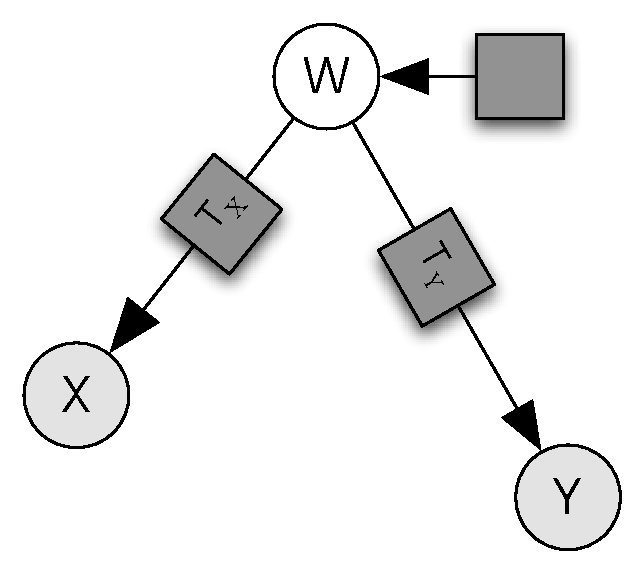
\includegraphics [scale=0.4] {figs/parent.pdf}
   \caption{
     \textbf{A simple example of transducer composition to build an
       evolutionary model of two extant sequences.}
    An ancestral sequence $W$ evolves into two descendant sequences $X$ and $Y$.
     A singlet transducer (the horizontal gray box) emits an ancestral sequence and structure
     and two branch transducers (the gray boxes labeled $T_X$ and $T_Y$)
     mutate it according to the specified evolutionary model.
     Gray nodes correspond to observed data and white nodes unobserved data.
   }
   \figlabel{parent}
 \end{figure}
 
 \begin{figure}[!ht]
   \centering
 %  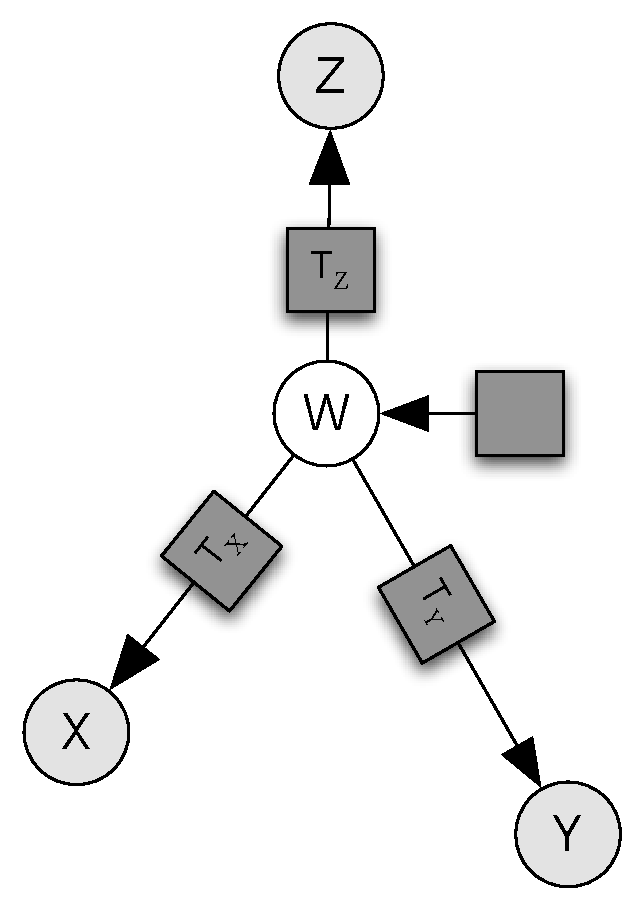
\includegraphics [scale=0.4] {figs/threeway.pdf}
   \caption{
     \textbf{Transducer composition on a star phylogeny with three
       (extant) leaf sequences.}
     An ancestral sequence $W$ evolves into three descendant sequences $X$, $Y$ and $Z$.
     A singlet transducer (the horizontal gray box) emits an ancestral sequence and structure
     and three branch transducers (the gray boxes labeled $T_X$, $T_Y$ and $T_Z$)
     mutate it according to the specified evolutionary model.
     Gray nodes correspond to observed data and white nodes unobserved data.
     If the branch transducers are time-reversible, then this star phylogeny with three leaves is
     the neighborhood of any interior node in a (binary) phylogenetic tree, 
     from which it follows that evaluating the likelihood function
     on this star phylogeny is sufficient, in principle, for a sampling algorithm on an arbitrary phylogeny.
   }
\figlabel{threeway}
 \end{figure}
 
\begin{figure}[!ht]
  \centering
%  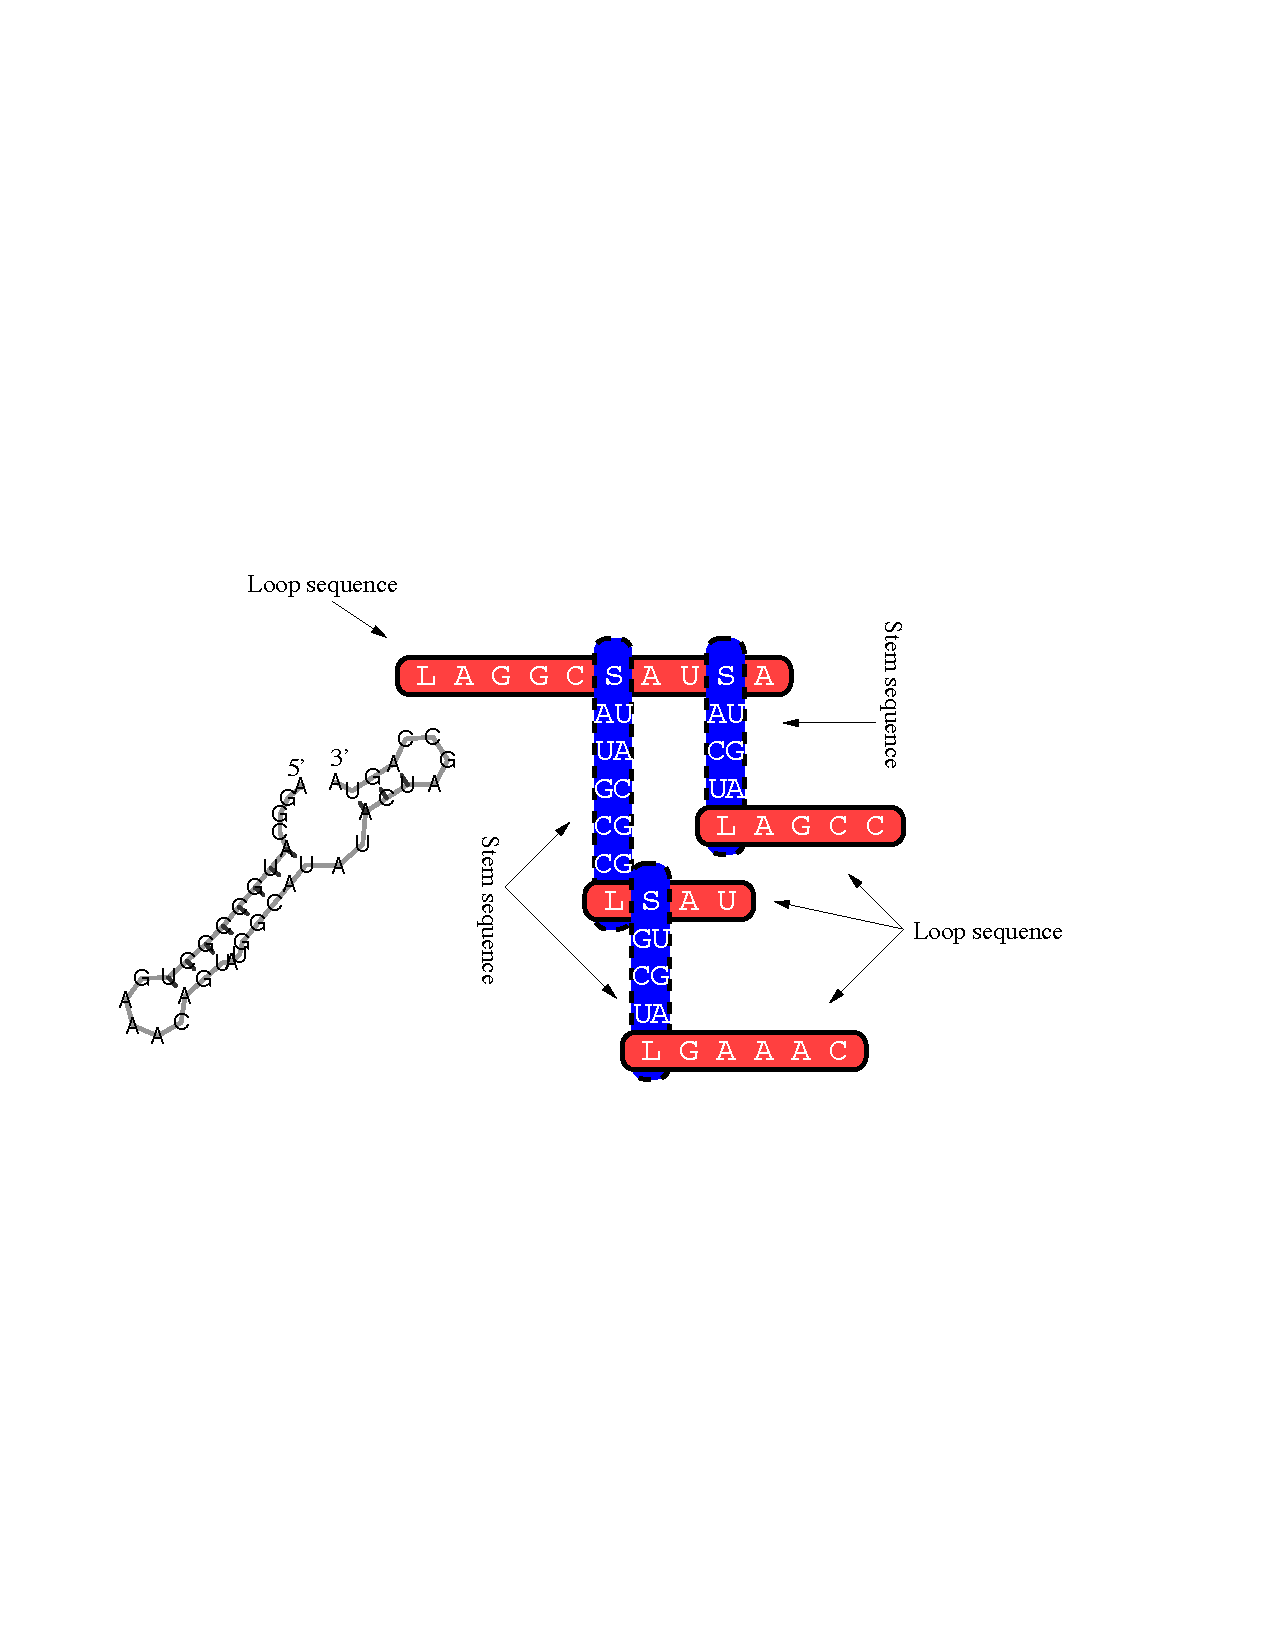
\includegraphics [width=0.5\textwidth] {figs_plos/stree-with-structure.pdf}
  \caption{
    \textbf{The TKF Structure Tree model represents the
      evolution of RNA structure as nested stem and loop sequences.}
    The model consists of recursively nested loop sequences (gray,
    horizontal) and stem sequences (black, vertical). The loops are
    sequences of unpaired bases and the stems are sequences of
    covarying base-pairs. Both loop and stem sequences evolve
    according to the Thorne-Kishino-Felsenstein (TKF) model
    \cite{ThorneEtal91} of molecular evolution.  Figure is extended
    from a similar version in \cite{Holmes2004}.
  }
  \figlabel{tkfst}
\end{figure}

\begin{figure}[!ht]
  \centering
%  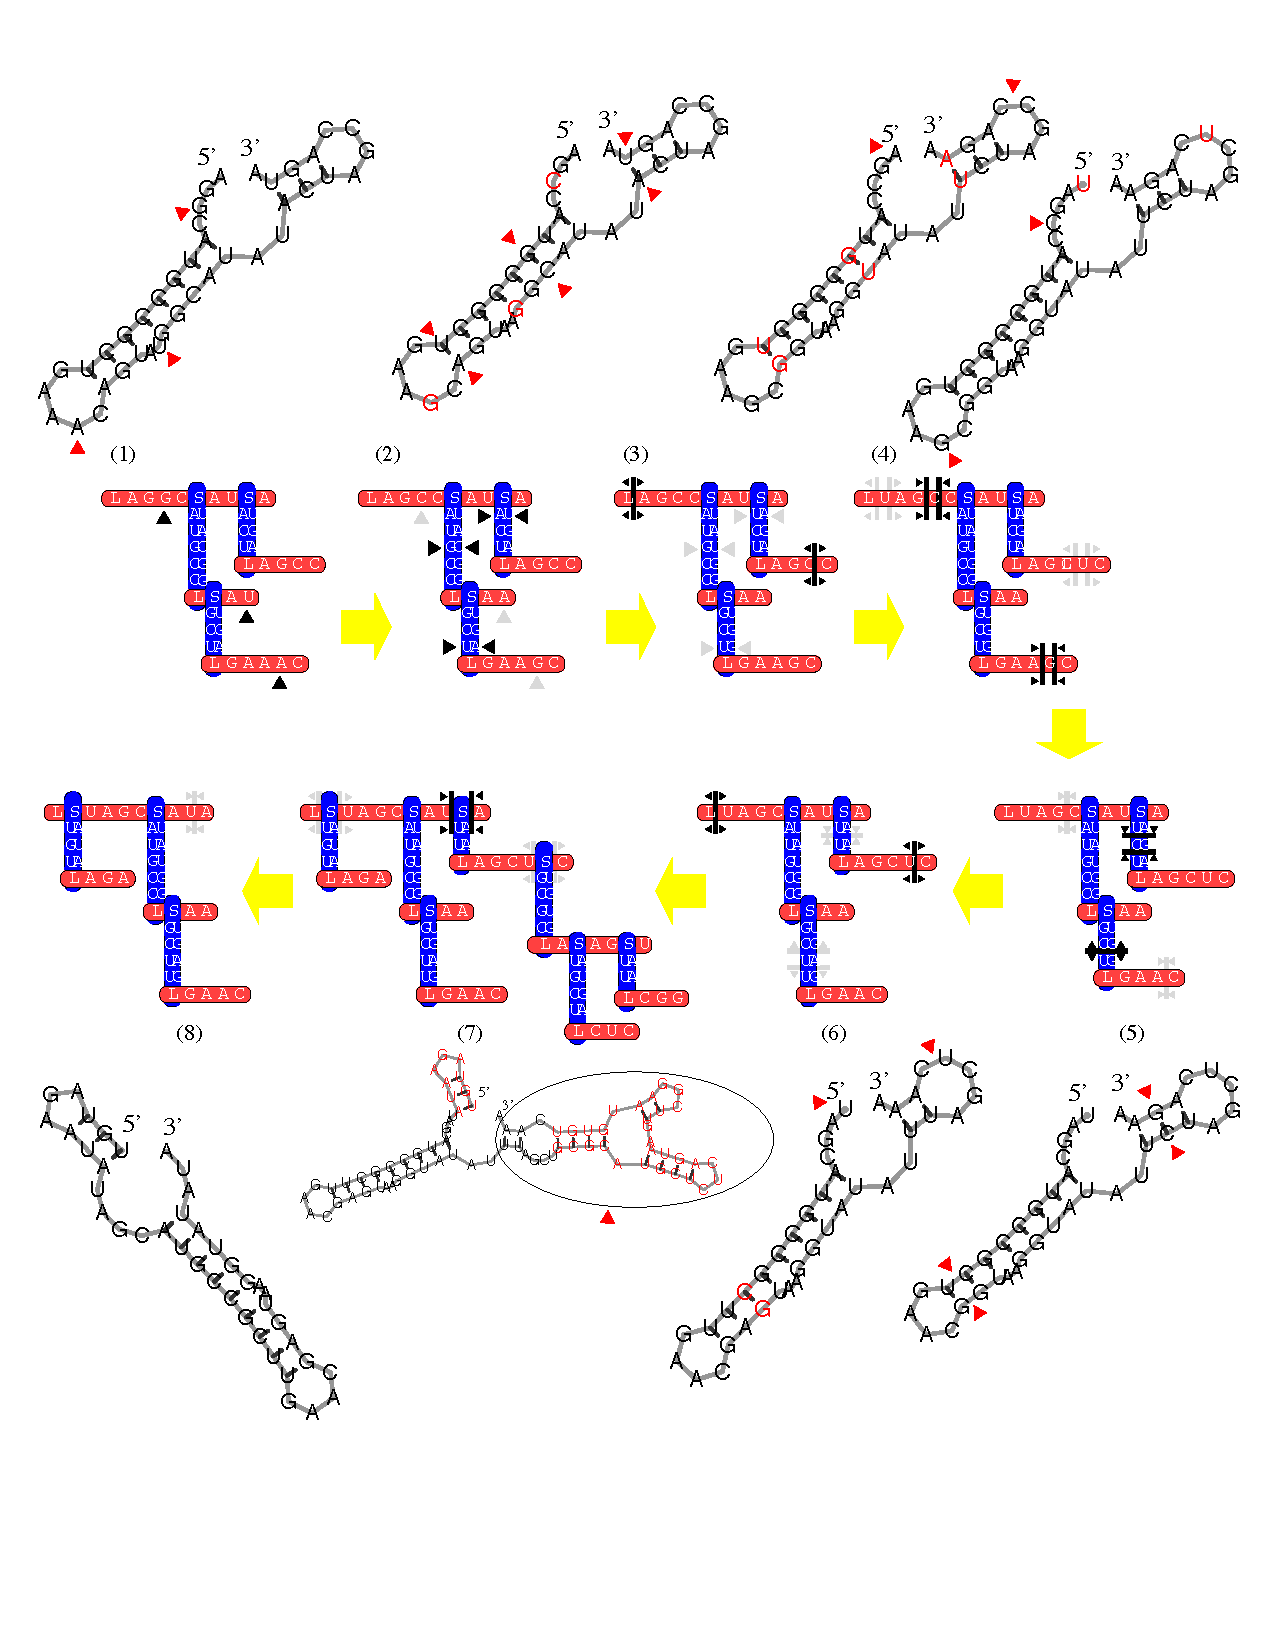
\includegraphics [width=0.5\textwidth] {figs_plos/stree-mutations-with-structures.pdf}
  \caption{
    \textbf{Evolution of a RNA structure under the TKF Structure Tree
      model.}
    The TKF Structure Tree model includes phenomena such as point
    mutations in loop sequences ($1 \rightarrow 2$ and $4 \rightarrow 5$), covariant
    mutations in stem sequences ($2 \rightarrow 3$), insertions in
    loop sequences ($3 \rightarrow 4$), insertions in stem sequences
    ($5 \rightarrow 6$), structural insertions ($6 \rightarrow 7$),
    and structural deletions ($7 \rightarrow 8$).
   Figure is extended from a similar version in \cite{Holmes2004}.
  }
  \figlabel{tkfst-mutations}
\end{figure}

% figure produced automatically with simulations/plots.r from simulations/inferred/indiegram.analysis
\begin{figure}[!ht]
  \centering
  % 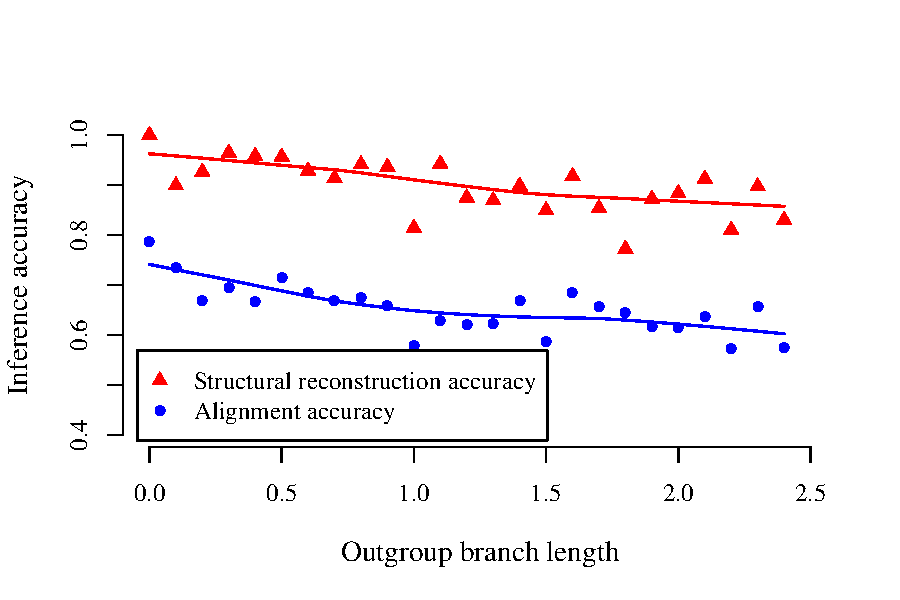
\includegraphics[width=5in]{figs_plos/simulations.pdf}
  \caption{
    \textbf{Dependence of reconstruction accuracy on outgroup branch
      length.}
    We investigated the dependence of structural reconstruction and
    alignment accuracy on outgroup branch length by simulating the
    evolution of three structural RNAs under our model.  The two
    sister species were equidistant from the ancestral sequence, with
    a branch length of 1, corresponding to one expected
    substitution per site in loop sequence.  We allowed the outgroup
    branch length to vary between $[0, 2.5]$.  We divided this interval
    into 25 bins and simulated 25 alignments for each bin.
    Parameters used were $\lambda_l = 0.025$ and $\mu_l = 0.03$ for
    loop sequence and $\lambda_l = 0.007$ and $\mu_l = 0.01$ for stem
    sequence; the probability of a stem insertion was $0.1$.  These
    yielded a mean loop length of 5 bp and a mean stem length of 2.33 bp,
    with $\sim 0.3$ substructure indels per alignment.
    We selected challenging alignments to reconstruct by requiring
    that there be at least two ancestral stems, loops of length $\in [3,
    10]$ bp and stems of length $\in [1, 20]$ bp; to reduce the complexity of
    our algorithms we additionally required that the sequences have
    lengths $\in [30, 70]$ bp.
    ``Structural reconstruction accuracy'' is the fraction of
    base-pairs in the ancestral structure present in the
    maximum-likelihood reconstruction thereof; ``Alignment accuracy''
    is a measure of sequence alignment accuracy which takes both
    aligned and unaligned (indels) nucleotides into account,
    qualitatively corresponding to giving equal weight to sensitivity
    and specificity (see
    \cite{SchwartzMyersPachter2006} for a precise definition).
}
  \figlabel{simulations}
\end{figure}


\clearpage
\section*{Tables}

\begin{table}[!ht]
  \caption{
    \textbf{State types of the singlet transducer (single-sequence
      SCFG) of the TKF Structure Tree model.}}
  \begin{tabular}{|l|rrrl|}
    \hline
    State & $\type$ & $\absorb$ & $\emit$ & description \\ \hline
    $L$ & $\Sstart$ & & & Start of a loop \\ \hline
    $I_L$ & $\Sinsert$ & & $(x,\Tnull)$ & Single-base emission \\ \hline \hline
    $S$ & $\Sstart$ & & & Start of a stem \\ \hline
    $I_S$ & $\Sinsert$ & & $(x,y)$ & Base-pair emission \\ \hline \hline
    $B$ & $\Sinsert$ & & $(L\,S)$ & Bifurcation \\ \hline
  \end{tabular}
  \begin{flushleft}
    Singlet transducers can only have states of type $\Sstart$ or
    $\Sinsert$.
  \end{flushleft}
 \tablabel{tkfstsinglet-types}
\end{table}


% Use table to allow the table to span the width of the entire page.
\begin{table}[!ht]
  \caption{
    \textbf{Singlet transducer (single-sequence SCFG) of the TKF Structure Tree model.}}
  \begin{tabular}{|rcl|r||rcl|r|}
    \hline
    Source & $\rightarrow$ & Destination & probability & Source & $\rightarrow$ & Destination & probability \\ \hline
    $L$ & $\rightarrow$ & $u \,\, I_L$ & $\kappa_l \cdot \pi_l(u)$ & $S$ & $\rightarrow$ & $u \,\, I_S \,\, v$ & $\kappa_s \cdot \pi_s(uv)$ \\ \hline
    & $|$ & $B$ & $\kappa_l \cdot \pi_l(S)$ & & $|$ & $B_e$ & $1-\kappa_s$ \\ \hline
    & $|$ & $\Send$ & $1-\kappa_l$ & & & & \\ \hline
    $I_L$ & $\rightarrow$ & $u \, \, I_L$ & $\kappa_l \cdot \pi_l(u)$ & $I_S$ & $\rightarrow$ & $u \,\, I_S \,\, v$ & $\kappa_s \cdot \pi_s(uv)$\\ \hline
    & $|$ & $B$ & $\kappa_l \cdot \pi_l(S)$ & & $|$ & $B_e$ & $1-\kappa_s$\\ \hline
    & $|$ & $\Send$ & $1-\kappa_l$ & & & & \\ \hline \hline
    $B$ & $\rightarrow$ & $(L \,\, S)$ & 1 & & & & \\ \hline
    $B_e$ & $\rightarrow$ & $(L \,\, \Send)$ & 1 & & & & \\ \hline
  \end{tabular}
  \begin{flushleft}
    The state types for this model are shown in
    \tabref{tkfstsinglet-types}.  The singlet transducer generates
    ancestral RNA sequences and structures.  We use the notation of
    formal grammars to represent state transformation rules; for
    example, the rule $I_L \rightarrow u\,\,I_L$ corresponds to (in a
    Pair HMM) an $\Sinsert$ state $I_L$ emitting a nucleotide $u$ and
    then making a self-transition.  Both loop ($L$ and $I_L$) and stem
    ($S$ and $I_S$) sequence evolve as TKF sequences with length
    parameters $\kappa_l$ and $\kappa_s$ (defined in ``A simple model
    of RNA structural evolution'').  $\pi_l(u)$ and $\pi_s(uv)$ are
    the equilibrium distributions of unpaired nucleotides $u$ and
    paired nucleotides $(u,v)$ and are normalized such that
    $\pi_l(S) + \sum_u \pi_l(u) = 1$ and $\sum_{u,v} \pi_s(uv) = 1$.  The bifurcation state $B_e$ is used
    to end stem sequences (only loop sequences are allowed to
    transition to the empty string).
  \end{flushleft}
  \tablabel{tkfstsinglet}
\end{table}

\begin{table}[!ht]
  \caption{
    \textbf{State types of the branch transducer
      (conditionally-normalized Pair SCFG) of the TKF Structure Tree
      model.}}
  \begin{tabular}{|l|rrrl|} \hline
    State & $\type$ & $\absorb$ & $\emit$ & description \\ \hline
    $L$ & $\Sstart$ & & & Start of a loop \\ \hline
    $I_L$ & $\Sinsert$ & & $(u,\Tnull)$ & Single-base insertion \\ \hline
    $M_L$ & $\Smatch$ & $(x,\Tnull)$ & $(u,\Tnull)$ & Single-base substitution \\ \hline
    $D_L$ & $\Smatch$ & $(x,\Tnull)$ & & Single-base deletion \\ \hline
    $W_L$ & $\Swait$ & & & Wait for next base \\ \hline \hline
    $S$ & $\Sstart$ & & & Start of a stem \\ \hline
    $I_S$ & $\Sinsert$ & & $(u,v)$ & Base-pair insertion \\ \hline
    $M_S$ & $\Smatch$ & $(x,y)$ & $(u,v)$ & Base-pair substitution \\ \hline
    $D_S$ & $\Smatch$ & $(x,y)$ & & Base-pair deletion \\ \hline
    $W_S$ & $\Swait$ & & & Wait for next base-pair \\ \hline \hline
    $B_i$ & $\Sinsert$ & & $(L_i\,S_i)$ & Stem insertion \\ \hline
    $B$ & $\Smatch$ & $(L\,S)$ & $(L\,S)$ & Stem conservation \\ \hline
    $B_p$ & $\Smatch$ & $(L\,S)$ & $(L\,\Send)$ & Stem deletion \\ \hline
    $B_e$ & $\Smatch$ & $(L\,\Send)$ & $(L\,\Send)$ & Stem extinction \\ \hline
  \end{tabular}
  \begin{flushleft}
    States which have the same names as states of the singlet transducer in \tabref{tkfstsinglet-types}
    are the branch-transducer equivalents of the corresponding singlet-transducer states
    (e.g., a $\Smatch$ state might be the branch equivalent of an $\Sinsert$ state).
    States $L_i$ and $S_i$ are the $\Sstart$ states of a sub-model (not shown) identical
    in structure to the singlet transducer.  They are used to insert a
    new stem-loop structure.
  \end{flushleft}
  \tablabel{tkfstbranch-types}
\end{table}

% Use table to allow the table to span the width of the entire page.
\begin{table}[!ht]
  \caption{
    \textbf{Branch transducer (conditionally-normalized Pair SCFG) of
      the TKF Structure Tree model.}}
  \begin{tabular}{|rcl|r||rcl|r|} \hline
    Source & $\rightarrow$ & Destination & probability & Source & $\rightarrow$ & Destination & probability \\ \hline
    $L$ & $\rightarrow$ & $w \,\, I_L$ & $\beta_l(t) \cdot \pi_l(w)$ & $S$ & $\rightarrow$ & $w \,\, I_S \,\, x$ & $\beta_s(t) \cdot \pi_s(wx)$ \\ \hline
    & $|$ & $B_i$ & $\beta_l(t) \cdot \pi_l(S)$ & & $|$ & $W_S$ & $1-\beta_s(t)$ \\ \hline
    & $|$ & $W_L$ & $1-\beta_l(t)$ & & & &  \\ \hline
    $I_L$ & $\rightarrow$ & $w \,\, I_L$ & $\beta_l(t) \cdot \pi_l(w)$ & $I_S$ & $\rightarrow$ & $w \,\, I_S \,\, x$ & $\beta_s(t) \cdot \pi_s(wx)$ \\ \hline
    & $|$ & $B_i$ & $\beta_l(t) \cdot \pi_l(S)$ & & $|$ & $W_S$ & $1-\beta_s(t)$ \\ \hline
    & $|$ & $W_L$ & $1-\beta_l(t)$ & & & & \\ \hline
    $M_L$ & $\rightarrow$ & $w \,\, I_L$ & $\beta_l(t) \cdot \pi_l(w)$ & $M_S$ & $\rightarrow$ & $w \,\, I_S \,\, x$ & $\beta_s(t) \cdot \pi_s(wx)$ \\ \hline
    & $|$ & $B_i$ & $\beta_l(t) \cdot \pi_l(S)$ & & $|$ & $W_S$ & $1-\beta_s(t)$ \\ \hline
    & $|$ & $W_L$ & $1-\beta_l(t)$ & & & &  \\ \hline
    $D_L$ & $\rightarrow$ & $w \,\, I_L$ & $\gamma_l(t) \cdot \pi_l(w)$ & $D_S$ & $\rightarrow$ & $w \,\, I_S \,\, x$ & $\gamma_s(t) \cdot \pi_s(wx)$ \\ \hline
    & $|$ & $B_i$ & $\gamma_l(t) \cdot \pi_l(S)$ & & $|$ & $W_S$ & $1-\gamma_s(t)$ \\ \hline
    & $|$ & $W_L$ & $1-\gamma_l(t)$ & & & &  \\ \hline
    $W_L$ & $\rightarrow$ & $w \,\, M_L$ & $\alpha_l(t) \cdot M_l(u \rightarrow w)$ & $W_S$ & $\rightarrow$ & $w \,\, M_S \,\, x$ & $\alpha_s(t) \cdot M_s(uv \rightarrow wx)$ \\ \hline
    & $|$ & $D_L$ & $1-\alpha_l(t)$ & & $|$ & $D_S$ & $1-\alpha_s(t)$ \\ \hline
    & $|$ & $B$ & $\alpha_l(t)$ & & $|$ & $B_e$ & $1$ \\ \hline
    & $|$ & $B_p$ & $1-\alpha_l(t)$ & & & &  \\ \hline
    & $|$ & $\Send$ & $1$ & & & &  \\ \hline \hline
    $B$ & $\rightarrow$ & $L \,\, S$ & 1 & $B_p$ & $\rightarrow$ & $L \, \, \Send$ & 1 \\ \hline
    $B_i$ & $\rightarrow$ & $L_i \,\, S_i$ & 1 & $B_e$ & $\rightarrow$ & $L \, \, \Send$ & 1 \\ \hline \hline
  \end{tabular}
  \begin{flushleft}
    The state types for this model are shown in
    \tabref{tkfstbranch-types}. The branch transducer evolves a
    sequence and structure along a branch of the phylogenetic
    tree. States $L_i$ and $S_i$ are the $\Sstart$ states for a
    sub-model corresponding to an insertion of a new stem in the
    descendant sequences; the sub-model (not shown) is identical in
    structure to the singlet transducer shown in
    \tabref{tkfstsinglet}. $\pi_l(w)$ and $\pi_s(wx)$ are the
    equilibrium distributions of, respectively, descendant unpaired
    nucleotide $w$ and descendant paired nucleotides $(w,x)$;
    $M_l(u \rightarrow w)$ and $M_l(uv \rightarrow wx)$ are the conditional distributions
    (i.e., match probabilities) of a descendant unpaired
    nucleotide $w$ given an ancestral unpaired nucleotide $u$ and
    descendant paired nucleotides $(w,x)$ given ancestral nucleotides
    $(u,v)$. The functions $\alpha_{l,s}(t)$, $\beta_{l,s}(t)$ and
    $\gamma_{l,s}(t)$ are parametrized by the insertion and deletion rates
    of the TKFST model and are defined in ``A simple model of RNA
    structural evolution.''
  \end{flushleft}
  \tablabel{tkfstbranch}
\end{table}


% Tables created as follows:
% sort -k 1,2 bralibaseII.results | perl -pe 's/0\.(\d\d)(\d)\d+/$1.$2/g;s/ +/ & /g' | cols
% ...then manual editing

% Method                          & Metric      & U5   & g2intron & rRNA & tRNA & TPP_riboswitch
% stemloc.progressive             & Align_Sens  & 82.6 & 74.2     & 92.6 & 93.2 & 76.8          
% stemloc.progressive             & Align_ppv   & 83.7 & 74.8     & 92.8 & 93.9 & 80.7          
% stemloc.progressive             & Struct_Sens & 74.9 & 64.3     & 51.0 & 74.0 & 57.1          
% stemloc.progressive             & Struct_ppv  & 73.9 & 56.7     & 59.0 & 76.4 & 63.3          
% stemloc.progressive.xrate       & Align_Sens  & 82.6 & 74.2     & 92.6 & 93.2 & 76.8          
% stemloc.progressive.xrate       & Align_ppv   & 83.7 & 74.8     & 92.8 & 93.9 & 80.7          
% stemloc.progressive.xrate       & Struct_Sens & 90.5 & 88.2     & 77.2 & 88.5 & 72.3          
% stemloc.progressive.xrate       & Struct_ppv  & 66.2 & 63.2     & 64.4 & 70.6 & 74.7          
% stemloc.tkfst.progressive       & Align_Sens  & 81.6 & 75.4     & 91.4 & 94.6 & 62.4          
% stemloc.tkfst.progressive       & Align_ppv   & 81.7 & 75.0     & 92.6 & 94.4 & 73.7          
% stemloc.tkfst.progressive       & Struct_Sens & 37.9 & 42.1     & 37.4 & 70.9 & 36.2          
% stemloc.tkfst.progressive       & Struct_ppv  & 68.0 & 63.8     & 66.5 & 88.3 & 77.2          
% stemloc.tkfst.progressive.xrate & Align_Sens  & 81.6 & 75.4     & 91.4 & 94.6 & 62.4          
% stemloc.tkfst.progressive.xrate & Align_ppv   & 81.7 & 75.0     & 92.6 & 94.4 & 73.7          
% stemloc.tkfst.progressive.xrate & Struct_Sens & 80.8 & 84.5     & 80.6 & 88.6 & 59.8          
% stemloc.tkfst.progressive.xrate & Struct_ppv  & 60.7 & 64.1     & 66.9 & 71.1 & 63.9          

% We first modified \stemloc\ to allow the user to specify the Pair SCFG that it uses for progressive alignment.
% We then used our program \evoldoer, an implementation of TKFST for pairwise alignment,
% to generate Pair SCFGs corresponding to the TKFST model at timepoints $\{0.01,0.1,0.2,0.3,0.4\}$,
% using loop and stem substitution rate matrices estimated with \xrate\ from
% ribosomal RNA alignments \cite{DeRijkEtAl2001,DowellEddy2006}
% and TKFST parameters $\{\lambda_n,\mu_n\}$ estimated previously \cite{Holmes2004}.

\begin{table}[ht]
  \caption{
    \textbf{Percentage sensitivity and positive predictive value (Sensitivity / PPV) for pairwise nucleotide-level alignments in the \bralibaseII\ benchmark.}}
  \begin{tabular}{|r|rrrr|}
    \hline
    & U5                      & g2intron                & rRNA                    & tRNA \\
    \hline
    TKFST grammar     &      81.6  /      81.7  & {\bf 75.4} / {\bf
      75.0} &      91.4  /      92.6  & {\bf 94.6} / {\bf 94.4} \\ \hline
    \stemloc\ grammar & {\bf 82.6} / {\bf 83.7} &      74.2  /
    74.8  & {\bf 92.6} / {\bf 92.8} &      93.2  /      93.9 \\ \hline
    \end{tabular}
\begin{flushleft}
  We compared the performance of the TKFST model for progressive multiple alignment
  of RNAs against the performance of a grammar with a richer model of RNA structure (``\stemloc''; \cite{Holmes2005}).
  Sensitivity is defined as $\mbox{TP}/(\mbox{TP} + \mbox{FN})$ and PPV is defined as $\mbox{TP}/(\mbox{TP} + \mbox{FP})$,
  where TP is the number of true positives (correctly aligned residue pairs),
  FN is the number of false negatives (residue pairs that should have been aligned but were not) and
  FP is the number of false positives (residue pairs that were incorrectly aligned).
  These statistics are summed over all pairs of sequences in the multiple alignment;
  therefore, ``Sensitivity'' for pairwise residue alignments is equivalent to the Sum of Pairs Score or SPS \cite{ThompsonEtal99}.
  ``g2intron'' is the RFAM entry {\tt Intron\_gpII}, containing domains V and VI of the Group II intron.
  \end{flushleft}
  \tablabel{bralibaseII-align}
\end{table}

\begin{table}[ht]
  \caption{
    \textbf{Percentage sensitivity and positive predictive value (Sensitivity / PPV) for predicted base-pairs in the \bralibaseII\ benchmark.}}
  \begin{tabular}{|r|rrrr|}
    \hline
    & U5                      & g2intron                & rRNA                    & tRNA \\
    \hline
    TKFST grammar      &      37.9  /      68.0   &      42.1  /
    63.8  &      37.4  /      66.5  &      70.9  / {\bf 88.3} \\ \hline
    \stemloc\ grammar  &      74.9  / {\bf 73.9}  &      64.3  /
    56.7  &      51.0  /      59.0  &      74.0  /      76.4  \\ \hline
  \end{tabular}
  \begin{flushleft}
    We compared the performance of the TKFST model for structure-prediction accuracy during
    progressive multiple alignment of RNAs against the performance of a grammar with 
    a richer model of RNA structure (``\stemloc''; \cite{Holmes2005}).
    ``g2intron'' is the RFAM entry {\tt Intron\_gpII}, containing domains V and VI of the Group II intron.
  \end{flushleft}
  \tablabel{bralibaseII-struct}
\end{table}





% nanos: Counted 3672701 subseqs and 48323860 bifurcations.
% tRNA: Counted 12573792 subseqs and 404730480 bifurcations.
% Y: Counted 34474759 subseqs and 1429713088 bifurcations.
% g2intron: Counted 139037184 subseqs and 1895528744 bifurcations.
% Scaling constant is approximately
% A * (404730480 / 48323860) = (19 / 3) => A = 0.76
% time = A * (# bifs / # bifs for nanos) * time for nanos
% Y time = 0.76 * (1429713088 / 48323860) * 3 min = 67 min
% g2intron time = 0.76 * (1895528744 / 48323860) * 3 min = 89 min
\begin{table}[!ht]
  \caption{
   \textbf{Estimates of the memory and time required to reconstruct ancestral
     structures of three RNAs from several families of biological interest
     (as reported by \indiegram).}}
 \begin{tabular}{|l|rrr|} \hline
    Family & Sequence lengths & Memory & Time \\ \hline
    \emph{nanos} 3' TCE & 61-64 nt & 3 Gb & 3 min \\ \hline
    tRNA & 69-73 nt & 11 Gb & 19 min \\ \hline
    Y RNA & 47-81 nt & 33 Gb & 70 min \\ \hline
    Group II intron (domains V and VI) & 76-91 nt & 122 Gb & 90 min \\ \hline
  \end{tabular}
  \begin{flushleft}
    The \emph{nanos} 3' translational control element (TCE) sequences
    are the seed sequences of the
    corresponding RFAM family \cite{GriffithsJonesEtAl2003} and the
    three tRNA sequences are from the \bralibaseII\ database
    \cite{GardnerEtAl2005} (identifiers AB042432.1-14140\_14072,
    Z82044.1-16031\_16103 and AC008670.6-83725\_83795). The group II
    intron sequences (identifiers Z00044.1-87253\_87177,
    X57546.1-2817\_2907 and X04465.1-2700\_2775) are from BralibaseII
    \cite{GardnerEtAl2005}.  The Y RNAs are hY1, hY4, and hY5 from
    \cite{TeunissenEtAl2000}; sequence lengths exclude the conserved
    stem S1.  The time estimates are for a 2.2GHz AMD Opteron 848 CPU.
  \end{flushleft}
  \tablabel{complexities}
\end{table}


\clearpage
\section*{Algorithms}

\begin{algorithm}[!ht]
  \SetLine
  \SetKwFunction{rnd}{Random[0,1]}
  \KwIn{Rule $\rho'' \in \grules''$}
  \KwOut{Parse (sub)tree $T' \in \gtrees'$}

  \Switch{$\rho''$}{
    \Case{$X \to Y$}{
      \eIf{\rnd $< P(X \to Y) / q_{XY}$}{
        \KwRet{$(X \to Y)$} \;
      }{
        Let $z = \sum_W q_{XW} P'(W \to Y)$ \;
        Sample state $V$ from probability distribution $P(V) = q_{XV} P'(V \to Y) / z$ \;
        \KwRet{$(\mathrm{restoreTransitions}(X \to V) \to Y)$} \;
      }
    }
    \Case{$X \to \epsilon$}{
      \eIf{\rnd $< P'(X \to \epsilon) / P'(\epsilon | X)$}{
        \KwRet{$(X \to \epsilon)$} \;
      }{
        Let $z = \sum_W q_{XW} P'(W \to \epsilon)$ \;
        Sample state $V$ from probability distribution $P(V) = q_{XV} P'(V \to \epsilon) / z$ \;
        \KwRet{$(\mathrm{restoreTransitions}(X \to V) \to \epsilon)$} \;
      }
    }
    \Other{
      \KwRet{$(\rho'')$} \;
    }
  }
  \caption{\label{alg:restoreTransitions}
    Subroutine $\mathrm{restoreTransitions}(\rho'')$ for the null cycle elimination procedure.
  }
\end{algorithm}


\begin{algorithm}[!ht]
  \SetLine
  \SetKwFunction{rnd}{Random[0,1]}
  \KwIn{Rule $\rho' \in \grules'$}
  \KwOut{Parse (sub)tree $T \in \gtrees$}

  \Switch{$\rho'$}{
    \Case{$B^0 \to \epsilon$}{
      Let $B \to L\ R$ be the original bifurcation in $\grules$ \;
      $T_L \leftarrow \mathrm{sampleNullSubtree}(L)$ \;
      $T_R \leftarrow \mathrm{sampleNullSubtree}(R)$ \;
      \KwRet{$(B \to T_L\ T_R)$} \;
    }
    \Case{$B' \to L'$}{
      Let $B \to L\ R$ be the original bifurcation in $\grules$ \;
      $T_R \leftarrow \mathrm{sampleNullSubtree}(R)$ \;
      \KwRet{$(B \to L\ T_R)$} \;
    }
    \Case{$B' \to R'$}{
      Let $B \to L\ R$ be the original bifurcation in $\grules$ \;
      $T_L \leftarrow \mathrm{sampleNullSubtree}(L)$ \;
      \KwRet{$(B \to T_L\ R)$} \;
    }
    \Case{$B^2 \to L'\ R'$}{
      Let $B \to L\ R$ be the original bifurcation in $\grules$ \;
      \KwRet{$(B \to L\ R)$} \;
    }
    \lCase{$B^0 \to B'$}{
      \KwRet{$()$} \;
    }
    \lCase{$B' \to B^2$}{
      \KwRet{$()$} \;
    }
    \Other{
      Let $\rho$ be the original rule in $\grules$ \;
      \KwRet{$(\rho)$} \;
    }
  }

  \caption{\label{alg:restoreBifurcations}
    Subroutine $\mathrm{restoreBifurcations}(\rho')$ for the null cycle elimination procedure.
  }
\end{algorithm}


\begin{algorithm}[!ht]
  \SetLine
  \SetKwFunction{rnd}{Random[0,1]}
  \KwIn{Nonterminal $A \in \gnons$}
  \KwOut{Parse tree $T \in \gtrees: \mathrm{seq}(T) = \epsilon, \mathrm{root}(T) = A$}

  \eIf{$A$ is a bifurcation state, $A \to X\ Y$,}{
    $T_X \leftarrow \mathrm{sampleNullSubtree}(X)$ \;
    $T_Y \leftarrow \mathrm{sampleNullSubtree}(Y)$ \;
    \KwRet{$(A \rightarrow T_X\ T_Y)$} \;
  }{
    \eIf{\rnd $< P(A \to \epsilon) / P(\epsilon|A)$}{
      \KwRet{$(A \to \epsilon)$} \;
    }{
      Let $z = \sum_Y P(A \to Y) P(\epsilon | Y)$ \;
      Sample state $X$ from probability distribution $P(X) = P(A \to X) P(\epsilon | X) / z$ \;
      $T_X \leftarrow \mathrm{sampleNullSubtree}(X)$ \;
      \KwRet{$(A \rightarrow T_X)$} \;
    }
  }

  \caption{\label{alg:sampleNullSubtree}
    Subroutine $\mathrm{sampleNullSubtree}(A)$ for the null cycle elimination procedure.
  }
\end{algorithm}

\begin{algorithm}[!ht]

  \SetKwData{bifurcProb}{bifurcProb}
  \SetKwFunction{calcTransEmitProb}{calcTransEmitProb}
  \SetKwFunction{calcLBifurcProb}{calcLBifurcProb}
  \SetKwFunction{calcRBifurcProb}{calcRBifurcProb}
  \SetLine
  \KwIn{sequences $X, Y, Z$}

  \ForEach(\tcc*[f]{inside-outside sorted}){$n^{(X)} \in \foldenv^{(X)}$} {
    \ForEach(\tcc*[f]{inside-outside sorted}){$n^{(Y)} \in \foldenv^{(Y)}$} {
      \ForEach(\tcc*[f]{inside-outside sorted}){$n^{(Z)} \in \foldenv^{(Z)}$} {
        \BlankLine
        \ForEach{state $\bvec{a}$}{
          \BlankLine
          \bifurcProb $\leftarrow 0$\;
          \ForEach{$\left( n^{(X)}_L,n^{(X)}_R \right) \in b_{in}\left( n^{(X)} \right)$} {
            \ForEach{$\left( n^{(Y)}_L,n^{(Y)}_R \right) \in b_{in}\left( n^{(Y)} \right)$} {
              \ForEach{$\left( n^{(Z)}_L,n^{(Z)}_R \right) \in b_{in}\left( n^{(Z)} \right)$} {
                \bifurcProb += \calcLBifurcProb($\bvec{a}; \cdot$)\;
                \bifurcProb += \calcRBifurcProb($\bvec{a}; \cdot$)\;
              }
            }
          }
          \BlankLine
          $\alpha_{\bvec{a}} \left( n^{(X)}, n^{(Y)}, n^{(Z)} \right)$ $\leftarrow$ \calcTransEmitProb$\left( \bvec{a}; n^{(X)}, n^{(Y)}, n^{(Z)} \right)$\;
          $\alpha_{\bvec{a}} \left( n^{(X)}, n^{(Y)}, n^{(Z)} \right)$ += \bifurcProb\;
          store $\alpha_{\bvec{a}} \left( n^{(X)}, n^{(Y)}, n^{(Z)} \right)$\;
        }
        \BlankLine
      }
    }
  }
  \KwRet{$\alpha_{\bvec{a}}\left( n^{(X)}[0,L^{(X)}],n^{(Y)}[0,L^{(Y)}],n^{(Z)}[0,L^{(Z)}] \right)$}\;
  
  \caption{\alglabel{inside}
    The constrained Inside algorithm for three sequences $X, Y, Z$.
    Ensemble states $\bvec{a}$ in the iteration over states are sorted in Inside fill order
    with $\Semit$ states first, then $\Snull$ states in reverse topological order.
  }
\end{algorithm}

\begin{algorithm}[!ht]
  \SetKwData{emitProb}{emitProb}
  \SetLine
  \KwIn{state $\bvec{a}, n^{(X)}, n^{(Y)}, n^{(Z)}$, intermediate Inside matrix $\alpha$}

  \emitProb $\leftarrow 0$\;
  \ForEach{$\bvec{b} : \exists \,\bvec{a} \to \bvec{b}$} {
    \emitProb += $P \left( \bvec{a} \to \bvec{b} \right)\, \alpha_{\bvec{b}}\left( n^{(X)}, n^{(Y)}, n^{(Z)} \right)$\;
  }
  \ForEach{$\bvec{b} : \exists \,\bvec{a} \to \bvec{l}\,\bvec{b}\,\bvec{r}$} {
    \lIf{$c_{in}\left(\bvec{b}; n^{(X)}\right) \notin \foldenv^{(X)}$ or $c_{in}\left(\bvec{b}; n^{(Y)}\right) \notin \foldenv^{(Y)}$ or $c_{in}\left(\bvec{b}; n^{(Z)}\right) \notin \foldenv^{(Z)}$}{next\;}
    \emitProb += $P \left( \bvec{a} \to \bvec{l}\,\bvec{b}\,\bvec{r} \right)\, \alpha_{\bvec{b}}\left( c_{in}\left(\bvec{b}; n^{(X)}\right), c_{in}\left(\bvec{b}; n^{(Y)}\right), c_{in}\left(\bvec{b}; n^{(Z)}\right) \right)$\;
  }
  \KwRet{\emitProb}\;
  \caption{\alglabel{insidetransemit}
    Subroutine $\mathrm{calcTransEmitProb}()$ for the Inside algorithm.
    $\bvec{a}$ and $\bvec{b}$ are ensemble states; $\bvec{l}$ and $\bvec{r}$ are left and right terminal emissions.
  }
\end{algorithm}

\begin{algorithm}[!ht]

  \SetKwData{maxProb}{maxProb}
  \SetKwData{bifurcProb}{bifurcProb}
  \SetKwFunction{calcTransEmitProb}{calcTransEmitProb}
  \SetKwFunction{calcLBifurcProb}{calcLBifurcProb}
  \SetKwFunction{calcRBifurcProb}{calcRBifurcProb}
  \SetLine
  \KwIn{sequences $X, Y, Z$}

  \ForEach(\tcc*[f]{inside-outside sorted}){$n^{(X)} \in \foldenv^{(X)}$} {
    \ForEach(\tcc*[f]{inside-outside sorted}){$n^{(Y)} \in \foldenv^{(Y)}$} {
      \ForEach(\tcc*[f]{inside-outside sorted}){$n^{(Z)} \in \foldenv^{(Z)}$} {
        \BlankLine
        \ForEach{state $\bvec{a}$}{
          \BlankLine
          \bifurcProb $\leftarrow 0$\;
          \ForEach{$\left( n^{(X)}_L,n^{(X)}_R \right) \in b_{in}\left( n^{(X)} \right)$} {
            \ForEach{$\left( n^{(Y)}_L,n^{(Y)}_R \right) \in b_{in}\left( n^{(Y)} \right)$} {
              \ForEach{$\left( n^{(Z)}_L,n^{(Z)}_R \right) \in b_{in}\left( n^{(Z)} \right)$} {
                \bifurcProb += \calcLBifurcProb($\bvec{a}; \cdot$)\;
                \bifurcProb += \calcRBifurcProb($\bvec{a}; \cdot$)\;
              }
            }
          }
          \BlankLine
          $\gamma_{\bvec{a}} \left( n^{(X)}, n^{(Y)}, n^{(Z)} \right)$ \\
          $\qquad \leftarrow \max \left( \calcTransEmitProb \left( \bvec{a}; n^{(X)}, n^{(Y)}, n^{(Z)} \right), \bifurcProb \right)$ \;
          store $\gamma_{\bvec{a}} \left( n^{(X)}, n^{(Y)}, n^{(Z)} \right)$\;
        }
        \BlankLine
      }
    }
  }
  \KwRet{$\gamma_{\bvec{a}}\left( n^{(X)}[0,L^{(X)}],n^{(Y)}[0,L^{(Y)}],n^{(Z)}[0,L^{(Z)}] \right)$}\;
  
  \caption{\alglabel{cyk}
    The constrained CYK algorithm for three sequences $X, Y, Z$.
    Ensemble states $\bvec{a}$ in the iteration over states are sorted in Inside fill order
    with $\Semit$ states first, then $\Snull$ states in reverse topological order.
  }
\end{algorithm}

\begin{algorithm}[!ht]
  \SetKwData{emitProb}{emitProb}
  \SetLine
  \KwIn{state $\bvec{a}, n^{(X)}, n^{(Y)}, n^{(Z)}$, intermediate CYK matrix $\gamma$}

  \emitProb $\leftarrow 0$\;
  \ForEach{$\bvec{b} : \exists \,\bvec{a} \to \bvec{b}$} {
    \emitProb = $\max \left( \emitProb, P \left( \bvec{a} \to \bvec{b} \right)\, \gamma_{\bvec{b}}\left( n^{(X)}, n^{(Y)}, n^{(Z)} \right) \right)$\;
  }
  \ForEach{$\bvec{b} : \exists \,\bvec{a} \to \bvec{l}\,\bvec{b}\,\bvec{r}$} {
    \lIf{$c_{in}\left(\bvec{b}; n^{(X)}\right) \notin \foldenv^{(X)}$ or $c_{in}\left(\bvec{b}; n^{(Y)}\right) \notin \foldenv^{(Y)}$ or $c_{in}\left(\bvec{b}; n^{(Z)}\right) \notin \foldenv^{(Z)}$}{next\;}
    \emitProb = $\max \left( \emitProb, P \left( \bvec{a} \to \bvec{l}\,\bvec{b}\,\bvec{r} \right)\, \gamma_{\bvec{b}}\left( c_{in}\left(\bvec{b}; n^{(X)}\right), c_{in}\left(\bvec{b}; n^{(Y)}\right), c_{in}\left(\bvec{b}; n^{(Z)}\right) \right) \right)$\;
  }
  \KwRet{\emitProb}\;
  \caption{\alglabel{cyktransemit}
    Subroutine $\mathrm{calcTransEmitProb}()$ for the CYK algorithm.
    $\bvec{a}$ and $\bvec{b}$ are ensemble states; $\bvec{l}$ and $\bvec{r}$ are left and right terminal emissions.
  }
\end{algorithm}


\begin{algorithm}[!ht]
  \SetKwFunction{calcTransEmitProb}{calcTransEmitProb}
  \SetKwData{bifurcProb}{bifurcProb}
  \SetKwFunction{calcLBifurcProb}{calcLBifurcProb}
  \SetKwFunction{calcRBifurcProb}{calcRBifurcProb}
  \SetLine
  \KwIn{sequences $X, Y, Z$, Inside matrix $\alpha$}

  \ForEach(\tcc*[f]{outside-inside sorted}){$n^{(X)} \in \foldenv^{(X)}$} {
    \ForEach(\tcc*[f]{outside-inside sorted}){$n^{(Y)} \in \foldenv^{(Y)}$} {
      \ForEach(\tcc*[f]{outside-inside sorted}){$n^{(Z)} \in \foldenv^{(Z)}$} {
        \BlankLine
        \ForEach{state $\bvec{b}$}{
          \BlankLine
          \bifurcProb $\leftarrow 0$\;
          \ForEach{$\left( n^{(X)}_O,n^{(X)}_L \right) \in b_{out,L}\left( n^{(X)} \right)$}{
            \ForEach{$\left( n^{(Y)}_O,n^{(Y)}_L \right) \in b_{out,L}\left( n^{(Y)} \right)$}{
              \ForEach{$\left( n^{(Z)}_O,n^{(Z)}_L \right) \in b_{out,L}\left( n^{(Z)} \right)$}{
                \bifurcProb += \calcLBifurcProb($\bvec{b}; \cdot$)\;
              }
            }
          }
          \ForEach{$\left( n^{(X)}_O,n^{(X)}_R \right) \in b_{out,R}\left( n^{(X)} \right)$}{
            \ForEach{$\left( n^{(Y)}_O,n^{(Y)}_R \right) \in b_{out,R}\left( n^{(Y)} \right)$}{
              \ForEach{$\left( n^{(Z)}_O,n^{(Z)}_R \right) \in b_{out,R}\left( n^{(Z)} \right)$}{
                \bifurcProb += \calcRBifurcProb($\bvec{b}; \cdot$)\;
              }
            }
          }
          \BlankLine
          $\beta_{\bvec{b}} \left( n^{(X)}, n^{(Y)}, n^{(Z)} \right) \leftarrow$ \calcTransEmitProb$\left( \bvec{b}; n^{(X)}, n^{(Y)}, n^{(Z)} \right)$\;
          $\beta_{\bvec{b}} \left( n^{(X)}, n^{(Y)}, n^{(Z)} \right)$ += \bifurcProb\;
          store $\beta_{\bvec{b}} \left( n^{(X)}, n^{(Y)}, n^{(Z)} \right)$\;
        }
        \BlankLine
      }
    }
  }
  \caption{\alglabel{outside}
    The constrained Outside algorithm for three sequences $X, Y, Z$.
    Ensemble states $\bvec{a}$ in the iteration over states are sorted in Outside fill order
    with $\Semit$ states first, then $\Snull$ states in topological order.
  }
\end{algorithm}

\begin{algorithm}[!ht]
  \SetKwData{emitProb}{emitProb}
  \SetLine
  \KwIn{state $\bvec{b}, n^{(X)}, n^{(Y)}, n^{(Z)}$, intermediate Outside matrix $\beta$}

  \emitProb $\leftarrow 0$\;
  \ForEach{$\bvec{a} : \exists \,\bvec{a} \to \bvec{b}$} {
    \emitProb += $P \left( \bvec{a} \to \bvec{b} \right)\, \beta_{\bvec{a}}\left( n^{(X)}, n^{(Y)}, n^{(Z)} \right)$\;
  }
  \ForEach{$\bvec{a} : \exists \,\bvec{a} \to \bvec{l}\,\bvec{b}\,\bvec{r}$} {
    \lIf{$c_{out}\left(\bvec{b}; n^{(X)}\right) \notin \foldenv^{(X)}$ or $c_{out}\left(\bvec{b}; n^{(Y)}\right) \notin \foldenv^{(Y)}$ or $c_{out}\left(\bvec{b}; n^{(Z)}\right) \notin \foldenv^{(Z)}$}{next\;}
    \emitProb += $P \left( \bvec{a} \to \bvec{l}\,\bvec{b}\,\bvec{r} \right)\, \beta_{\bvec{a}}\left( c_{out}\left(\bvec{b}; n^{(X)}\right), c_{out}\left(\bvec{b}; n^{(Y)}\right), c_{out}\left(\bvec{b}; n^{(Z)}\right) \right)$\;
  }
  \KwRet{\emitProb}\;
  \caption{\alglabel{outsidetransemit}
    Subroutine $\mathrm{calcTransEmitProb}()$ for the Outside algorithm.
    $\bvec{a}$ and $\bvec{b}$ are ensemble states; $\bvec{l}$ and $\bvec{r}$ are left and right terminal emissions.
  }
\end{algorithm}

\begin{algorithm}[!ht]

  \SetKw{Select}{select}
  \SetKw{Pop}{pop}
  \SetKw{Push}{push}
  \SetKw{Goto}{goto}
  \SetKw{Mainloop}{main loop}
  \SetKwData{coordinateStack}{coordinateStack}
  \SetKwFunction{goto}{goto}
  \SetKwBlock{Begin}{begin main loop:}{end}
  \SetLine
  \KwIn{sequences $X, Y, Z$}

  pushdown stack coordinateStack; \tcc*[f]{hold (state, subsequence triplet) pairs} \\
  $\bvec{a} \leftarrow \Sstart$; \tcc*[f]{current ensemble state} \\
  $n^{(X)} \leftarrow N^{(X)}$; \tcc*[f]{current $X$ subsequence; $N^{(X)}$ is the outermost subsequence} \\
  $n^{(Y)} \leftarrow N^{(Y)}$; \tcc*[f]{current $Y$ subsequence; $N^{(Y)}$ is the outermost subsequence} \\
  $n^{(Z)} \leftarrow N^{(Z)}$; \tcc*[f]{current $Z$ subsequence; $N^{(Z)}$ is the outermost subsequence} \\
  clear \coordinateStack;\

  \Begin{
    output current state $\bvec{a}$ and subsequence triplet $\left( n^{(X)}, n^{(Y)}, n^{(Z)} \right)$\;
    \SetLine
    \uIf(\tcc*[f]{end of a parse subtree}){$\bvec{a}$ is the $\Send$ state}{
      \lIf(\tcc*[f]{end of the parse tree}){\coordinateStack is empty}{\Return}
      \Pop $\left( \bvec{a}, n^{(X)}, n^{(Y)}, n^{(Z)} \right)$ from \coordinateStack\;
      \Goto \Mainloop\;
    }
    \uElseIf(\tcc*[f]{bifurcation $\bvec{a} \to \bvec{c} \bvec{b}$}){$\bvec{a}$ is a bifurcation state}{
      \Select $\left( n^{(X)}_L, n^{(X)}_R \right) \in b_{in}\left( n^{(X)} \right)$,
      $\left( n^{(Y)}_L, n^{(Y)}_R \right) \in b_{in}\left( n^{(Y)} \right)$,
      $\left( n^{(Z)}_L, n^{(Z)}_R \right) \in b_{in}\left( n^{(Z)} \right)$ \\
      such that \\
      $\gamma_{\bvec{a}} \left(n^{(X)}, n^{(Y)}, n^{(Z)} \right) = \gamma_{\bvec{a}} \left(n^{(X)}_L, n^{(Y)}_L, n^{(Z)}_L \right)  \gamma_{\bvec{a}} \left(n^{(X)}_R, n^{(Y)}_R, n^{(Z)}_R \right)$ \;
      \Push $\left( \bvec{c}, n^{(X)}_R, n^{(Y)}_R, n^{(Z)}_R \right)$ onto \coordinateStack\;
      $\bvec{a} \leftarrow \bvec{b}$\;
      $n^{(X)} \leftarrow n^{(X)}_L$\;
      $n^{(Y)} \leftarrow n^{(Y)}_L$\;
      $n^{(Z)} \leftarrow n^{(Z)}_L$\;
      \Goto \Mainloop\;
    }
    \Else(\tcc*[f]{$\Semit$ or $\Snull$ state}){
      $m^{(X)} \leftarrow c_{in}\left(\bvec{b}; n^{(X)}\right)$ \;
      $m^{(Y)} \leftarrow c_{in}\left(\bvec{b}; n^{(Y)}\right)$ \;
      $m^{(Z)} \leftarrow c_{in}\left(\bvec{b}; n^{(Z)}\right)$ \;
      \Select $\bvec{b} \in \left\{ b : \exists \,\bvec{a} \to \bvec{l}\bvec{b}\bvec{r} \right\}$ \\
      such that \\
      $\gamma_{\bvec{a}} \left( n^{(X)}, n^{(Y)}, n^{(Z)} \right) = P(\bvec{a} \to \bvec{l}\bvec{b}\bvec{r}) \gamma_{\bvec{b}} \left( m^{(X)}, m^{(Y)}, m^{(Z)} \right)$\;
      $\bvec{a} \leftarrow \bvec{b}$\;
      $n^{(X)} \leftarrow m^{(X)}$\;
      $n^{(Y)} \leftarrow m^{(Y)}$\;
      $n^{(Z)} \leftarrow m^{(Z)}$\;
      \Goto \Mainloop\;
    }
  }
  \caption{\alglabel{cyktraceback}
    The constrained CYK traceback algorithm for three sequences $X, Y, Z$.
  }
\end{algorithm}





\end{document}

